\documentclass[11pt,a4paper]{article}

% ── Packages ──────────────────────────────────────────────────────
\usepackage[margin=2.5cm]{geometry}
\usepackage{graphicx}
\usepackage{booktabs}
\usepackage{amsmath}
\usepackage{hyperref}
\usepackage{xcolor}
\usepackage{float}
\usepackage{caption}
\usepackage{subcaption}
\usepackage{enumitem}
\usepackage{fancyhdr}
\usepackage{titlesec}
\usepackage{longtable}
\usepackage{array}
\usepackage{multirow}
\usepackage{pdflscape}
\usepackage[super]{natbib}
\usepackage{siunitx}

% ── Layout ────────────────────────────────────────────────────────
\pagestyle{fancy}
\fancyhf{}
\rhead{\small Reintroduction 2050}
\lhead{\small SSWD Evo-Epi Model}
\cfoot{\thepage}
\setlength{\parskip}{0.5em}
\setlength{\parindent}{0pt}

\hypersetup{
  colorlinks=true,
  linkcolor=blue!60!black,
  citecolor=blue!60!black,
  urlcolor=blue!60!black
}

% ── Custom colors ────────────────────────────────────────────────
\definecolor{alertred}{RGB}{180,30,30}
\definecolor{keyblue}{RGB}{30,80,160}

% ── Macros ───────────────────────────────────────────────────────
\newcommand{\rbar}{\ensuremath{\bar{r}}}
\newcommand{\scenario}[1]{\texttt{#1}}
\newcommand{\alertbox}[1]{%
  \begin{center}
  \fcolorbox{alertred}{alertred!8}{%
    \begin{minipage}{0.9\textwidth}
    \textcolor{alertred}{\textbf{Key Finding:}} #1
    \end{minipage}}
  \end{center}}

% ── Title ────────────────────────────────────────────────────────
\title{%
  \vspace{-1cm}
  {\Large\bfseries Captive-Bred Sunflower Star Reintroduction}\\[0.3em]
  {\large Full-Factorial Analysis of Resistance Genetics,\\
  Release Density, and Release Location}\\[0.5em]
  {\normalsize 40-Scenario Simulation: 2025\,--\,2050}
}
\author{%
  SSWD Evo-Epi Modeling Pipeline\\
  \small Prepared for Willem Weertman
}
\date{April 2026}

\begin{document}
\maketitle
\thispagestyle{fancy}

% ══════════════════════════════════════════════════════════════════
\section{Executive Summary}
% ══════════════════════════════════════════════════════════════════

This report presents results from a 40-scenario full-factorial reintroduction experiment for \textit{Pycnopodia helianthoides} (sunflower sea star), simulated under the SSWD evo-epi framework from 2025 to 2050. We crossed five resistance genetics profiles ($\times$\,4 release densities $\times$\,2 release locations) against a no-intervention baseline.

\textbf{The headline finding is counterintuitive and policy-critical:} releasing large numbers of low-resistance captive-bred animals actively \emph{harms} wild populations through competitive dilution of resistance alleles. At the highest release density (1000/site), pre-epidemic naive stock (R2, $\rbar=0.15$) drives Central California to functional extinction (CA-C\,=\,0.03\%), worse than the no-release baseline.

\medskip
\textbf{Key results:}
\begin{itemize}[nosep]
  \item \textbf{Breed for resistance, not numbers.} Only fully immune stock (R5, $\rbar=1.0$) achieves meaningful California recovery: CA-N\,=\,21.3\%, CA-C\,=\,14.6\%, CA-S\,=\,8.4\% at maximum density.
  \item \textbf{Competitive dilution is real and dangerous.} For R1--R3, increasing release density from 50 to 1000/site \emph{decreases} CA-C recovery by 94--98\%. The mechanism: naive animals compete for space and food but succumb to disease, diluting the genetic resistance of survivors.
  \item \textbf{No southward larval transport.} Washington releases (L2, Friday Harbor) produce zero California recovery---not even at R5/D4. Larval dispersal does not bridge the WA--CA gap.
  \item \textbf{Alaska is self-sustaining.} AK-PWS holds at 26.2--27.8\% across all 40 scenarios, indifferent to any intervention.
  \item \textbf{Diminishing returns above 200/site for high-resistance stock.} R5 gains only ${\sim}$2 percentage points moving from D2 (200/site) to D4 (1000/site) in CA-C, a 5$\times$ cost increase for marginal benefit.
\end{itemize}

\medskip
\textbf{Policy recommendation:} Captive breeding programs should prioritize selective breeding for SSWD resistance ($\rbar \geq 0.5$, ideally approaching 1.0) before any large-scale release. Mass release of unselected stock is not merely wasteful---it is actively harmful. If immune stock is unavailable, small-scale releases at $\leq$200/site using the best available survivors (R1, $\rbar=0.31$) represent the least-harmful interim strategy.


% ══════════════════════════════════════════════════════════════════
\section{Experimental Design}
% ══════════════════════════════════════════════════════════════════

\subsection{Model Framework}

All simulations use the SSWD evolutionary-epidemiological (evo-epi) metapopulation model. The model tracks \textit{Pycnopodia helianthoides} populations across 18 biogeographic regions spanning Baja California (BJ) to the western Aleutians (AK-AL), resolving individual-site dynamics within each region. The 18 regions, ordered south-to-north, are: BJ, CA-S, CA-C, CA-N, OR, WA-O, JDF, SS-S, SS-N, BC-C, BC-N, AK-FS, AK-FN, AK-OC, AK-PWS, AK-EG, AK-WG, and AK-AL.

\textbf{Disease dynamics.} Transmission follows a susceptible--infected (SI) framework with density- and temperature-dependent transmission coefficient $\beta(T, N)$. Temperature modulates pathogen virulence through a thermal performance curve, with SSWD severity increasing under marine heatwave conditions. Host mortality from infection is modulated by the individual's resistance allele value $r \in [0,1]$, where $r=0$ confers no resistance (pre-epidemic baseline) and $r=1.0$ confers complete immunity.

\textbf{Evolutionary dynamics.} Host resistance evolves through heritable allele frequencies subject to selection by SSWD mortality. Each individual carries a resistance value drawn from a distribution with mean $\rbar$ and variance determined by genetic diversity parameters. Individuals with higher $r$ survive disease exposure at higher rates, shifting the population's $\rbar$ upward over generations. This process captures the real-world observation that surviving \textit{Pycnopodia} populations show elevated resistance relative to pre-epidemic baselines.

\textbf{Dispersal.} Larval dispersal connects sites via an oceanographic connectivity matrix derived from Lagrangian particle-tracking simulations. The matrix encodes probabilities of larval transport between all site pairs, reflecting ocean current patterns in the Northeast Pacific. Critically, the matrix shows strong northward transport along the California Current but minimal southward transport, a feature that drives several key results in this experiment.

\textbf{Demographics.} Local population dynamics follow logistic growth with carrying capacity $K=1000$ per site. The reference population $K_\text{ref}=5000$ is used for normalizing recovery fractions. Reproduction, natural mortality, and density-dependent regulation operate on annual timesteps with monthly disease dynamics.

All scenarios use seed 42 for stochastic reproducibility. Reintroduction scenarios branch from the baseline forecast at simulation year 13 (calendar year 2025) and run to year 38 (2050), covering 25 years of post-release population dynamics.

\subsection{Factorial Design}

The experiment is a fully crossed $5 \times 4 \times 2 = 40$ factorial design (Table~\ref{tab:design}).

\begin{table}[H]
\centering
\caption{Factorial design: three experimental factors and their levels.}
\label{tab:design}
\begin{tabular}{llll}
\toprule
\textbf{Factor} & \textbf{Level} & \textbf{Label} & \textbf{Value} \\
\midrule
\multirow{2}{*}{Location} & L1 & Monterey, CA & All 238 CA sites \\
                           & L2 & Friday Harbor, WA & All JDF sites \\
\midrule
\multirow{5}{*}{Resistance} & R1 & CA-2025 survivors & $\rbar = 0.31$ \\
                             & R2 & Pre-epidemic naive & $\rbar = 0.15$ \\
                             & R3 & Mid-epidemic 2019  & $\rbar = 0.20$ \\
                             & R4 & Artificially selected & $\rbar = 0.50$ \\
                             & R5 & Immune & $\rbar = 1.00$ \\
\midrule
\multirow{4}{*}{Density}  & D1 & Low & 50/site \\
                           & D2 & Moderate & 200/site \\
                           & D3 & High & 500/site \\
                           & D4 & Saturation & 1000/site $(=K)$ \\
\bottomrule
\end{tabular}
\end{table}

The resistance levels represent plausible captive-breeding outcomes:
\begin{itemize}[nosep]
  \item \textbf{R1} ($\rbar=0.31$): Breeding from wild-caught California survivors---the best stock currently available. These animals have undergone natural selection through SSWD exposure since 2013.
  \item \textbf{R2} ($\rbar=0.15$): Breeding from pre-epidemic museum/aquarium stock with no SSWD selection history. This represents a ``genetic rescue'' scenario using maximum available genetic diversity.
  \item \textbf{R3} ($\rbar=0.20$): Intermediate selection---animals collected mid-epidemic (2019) before selection was complete.
  \item \textbf{R4} ($\rbar=0.50$): Artificially selected stock after multiple generations of managed breeding for resistance.
  \item \textbf{R5} ($\rbar=1.00$): Hypothetical fully immune stock, representing the upper bound of what resistance breeding could achieve. Serves as a benchmark.
\end{itemize}

\subsection{Baseline Reference}

The no-intervention baseline (F01) projects \textit{Pycnopodia} populations forward from 2012 to 2050 without any reintroduction. By 2050, total metapopulation recovery reaches only 8.3\% of pre-epidemic levels, with California functionally extinct: CA-S\,=\,0.0\%, CA-C\,=\,0.0\%, CA-N\,=\,0.03\%. The Juan de Fuca region (JDF) persists at 7.2\%, while AK-PWS---the stronghold---holds at 27.0\%. This baseline represents the counterfactual against which all reintroduction scenarios are evaluated.


% ══════════════════════════════════════════════════════════════════
\section{Results}
% ══════════════════════════════════════════════════════════════════

% ── 3.1 Full Factorial Overview ──────────────────────────────────
\subsection{Full Factorial Overview}

Figure~\ref{fig:heatmap} presents the complete results as heatmaps for both release locations. The L1 (Monterey) panel shows a stark division: R1--R3 produce marginal CA recovery that \emph{degrades} at high density, while R4--R5 show positive density--response relationships. The L2 (Friday Harbor) panel confirms that Washington releases produce no California recovery regardless of genetics or density, but do enhance JDF populations when high-resistance stock is used.

The diagonal of failure running from R2/D4 (bottom-right) to R1/D4 is the competitive dilution zone---the most policy-relevant feature of the entire experiment.

\begin{figure}[H]
  \centering
  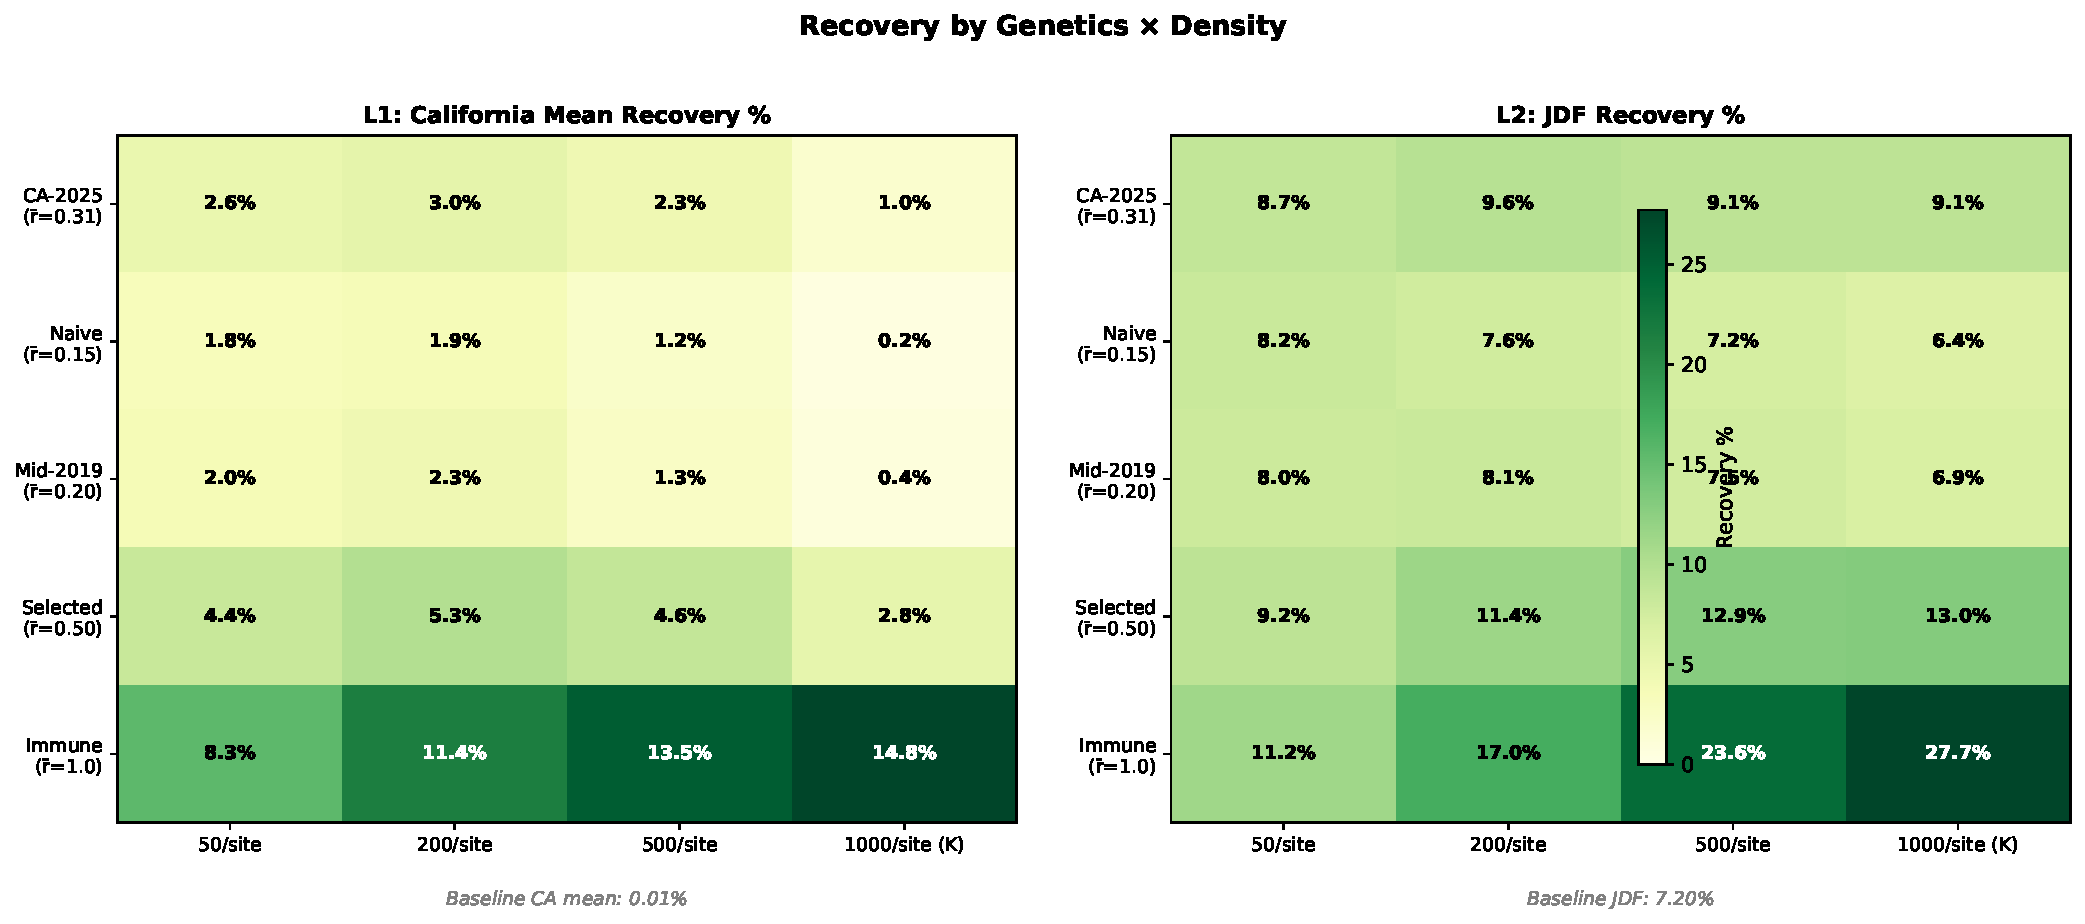
\includegraphics[width=\textwidth]{figures/fig_01_factorial_heatmap.pdf}
  \caption{\textbf{Full factorial heatmap across all 40 scenarios.} Recovery percentage by 2050 for each combination of resistance genetics (rows) and release density (columns), split by release location (L1: Monterey CA, L2: Friday Harbor WA). Warm colors indicate higher recovery. The critical pattern: for L1, low-resistance stocks (R1--R3) show declining recovery at high density, while only R5 achieves double-digit CA recovery. L2 scenarios show no CA spillover whatsoever.}
  \label{fig:heatmap}
\end{figure}


% ── 3.2 Baseline Comparison ─────────────────────────────────────
\subsection{Baseline Comparison}

Figure~\ref{fig:baseline} compares the baseline trajectory against the best-performing scenarios for each release location. The best L1 scenario (\scenario{L1\_R5\_D4}) lifts CA-C from 0.0\% to 14.6\% and CA-N from 0.03\% to 21.3\%---a transformative improvement contingent entirely on immune-level resistance. The best L2 scenario (\scenario{L2\_R5\_D4}) boosts JDF from 7.2\% to 27.7\%, nearly quadrupling the regional population, but contributes nothing to California.

Note that even the best scenario only recovers CA-C to ${\sim}$15\% of pre-epidemic levels. Full recovery of California populations likely requires either higher resistance, environmental improvement (reduced SST anomalies), or both.

\begin{figure}[H]
  \centering
  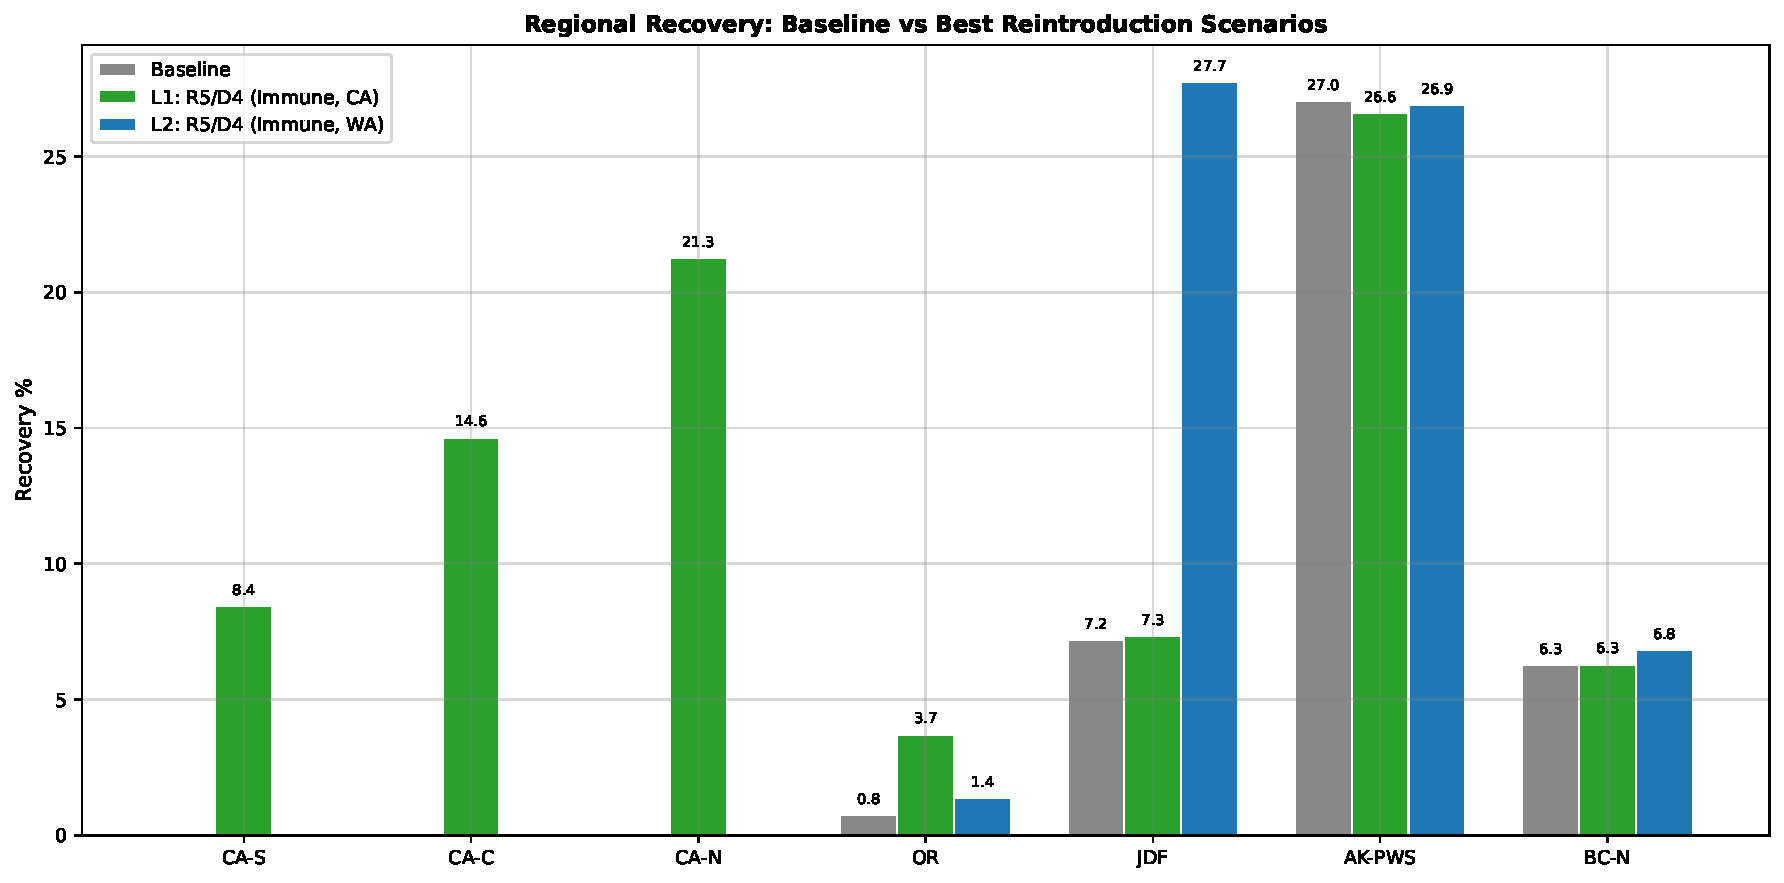
\includegraphics[width=\textwidth]{figures/fig_02_baseline_comparison.pdf}
  \caption{\textbf{Regional recovery comparison: baseline vs.\ best L1 and L2 scenarios.} The baseline (no intervention) maintains California at ${\sim}$0\% through 2050. The best L1 scenario (R5/D4, immune stock at saturation density into Monterey) achieves CA-N\,=\,21.3\% and CA-C\,=\,14.6\%. The best L2 scenario (R5/D4 into Friday Harbor) boosts JDF to 27.7\% but provides zero California benefit. AK-PWS is unchanged across all scenarios.}
  \label{fig:baseline}
\end{figure}


% ── 3.3 California Trajectories ─────────────────────────────────
\subsection{California Trajectories}

Figure~\ref{fig:ca_traj} tracks Central California (CA-C) population trajectories from 2012 to 2050 for selected scenarios. All trajectories show the initial SSWD crash (2013--2015), followed by divergence after the 2025 release. R5/D2 shows steady growth from release through 2050, reaching 12.3\%. R4/D2 achieves more modest recovery (5.4\%), while R1/D2 initially spikes post-release but then stagnates at 3.2\%---the dilution of resistance genetics prevents sustained growth even at moderate density.

The trajectory shapes are informative: R5 shows monotonic growth (resistance protects released animals, which then reproduce and build population), while R1 shows a characteristic ``release bump'' followed by gradual erosion as disease culls the susceptible stock.

\begin{figure}[H]
  \centering
  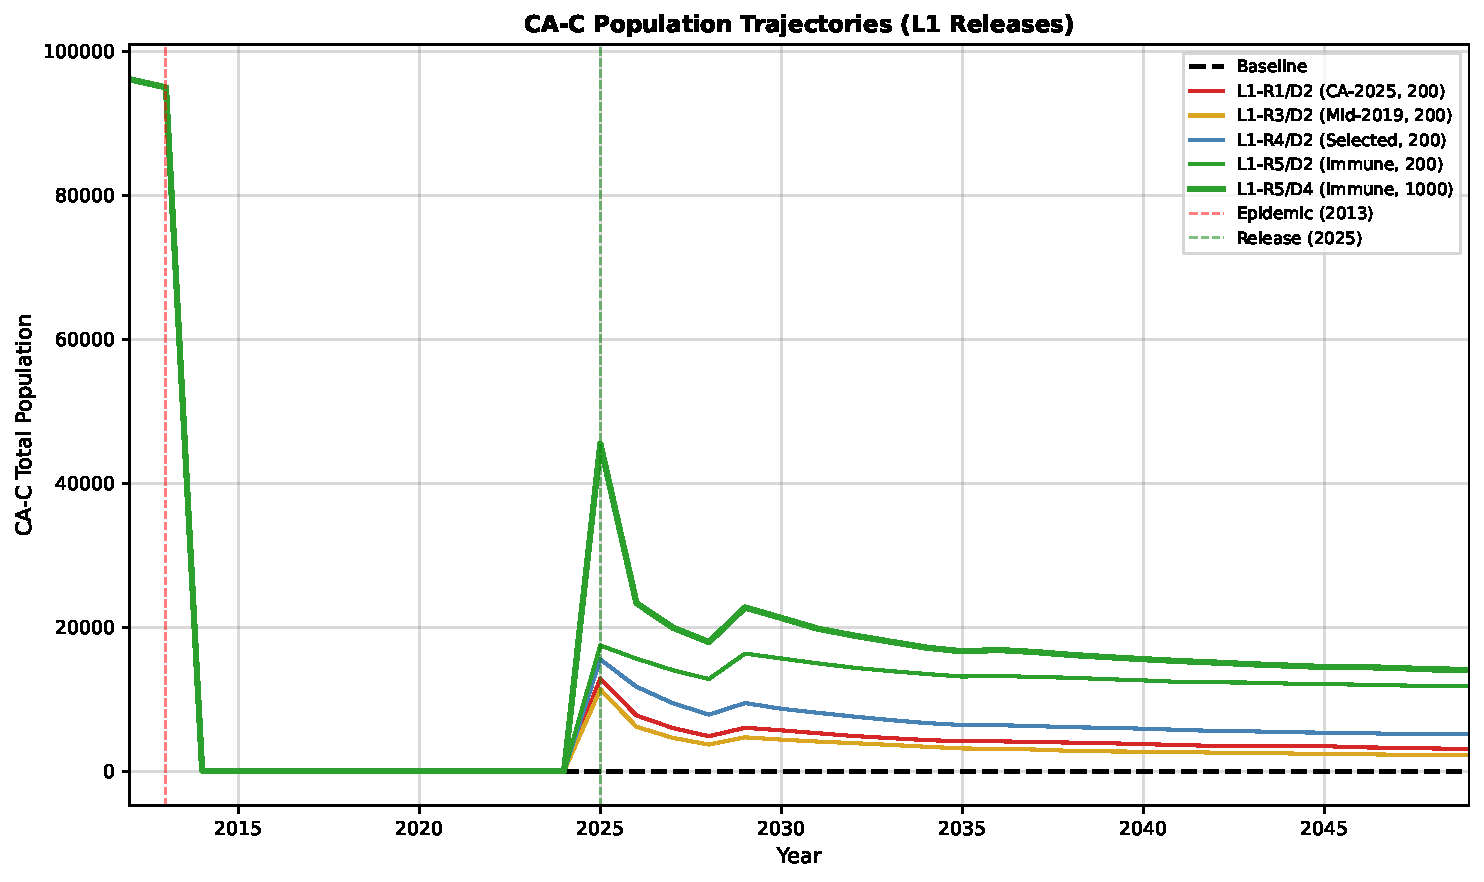
\includegraphics[width=\textwidth]{figures/fig_03_ca_trajectories.pdf}
  \caption{\textbf{CA-C population trajectories for R1, R4, and R5 at D2 (200/site), plus baseline.} All simulations show the SSWD crash (years 1--3). After the year-13 release, trajectories diverge: R5 (immune) shows sustained recovery reaching 12.3\% by 2050; R4 (selected) achieves moderate 5.4\%; R1 (survivors) stalls at 3.2\%. The baseline flatlines at 0\%. The post-release dynamics reveal the mechanism: resistant animals survive and reproduce, while susceptible stock dies off within years, providing only a transient numerical boost.}
  \label{fig:ca_traj}
\end{figure}


% ── 3.4 JDF Trajectories ────────────────────────────────────────
\subsection{Juan de Fuca Trajectories}

Figure~\ref{fig:jdf_traj} shows equivalent trajectories for the Juan de Fuca region under L2 (Friday Harbor) releases. JDF has a healthier baseline (7.2\%) than California, so the relative improvement from reintroduction is less dramatic but still substantial for high-resistance stock. R5/D4 reaches 27.7\%, while R5/D2 achieves 17.0\%.

The competitive dilution signal is weaker in JDF than in California, likely because the existing wild population is larger and more resistant (having survived ongoing SSWD pressure), making it harder for naive releases to overwhelm the resident gene pool.

\begin{figure}[H]
  \centering
  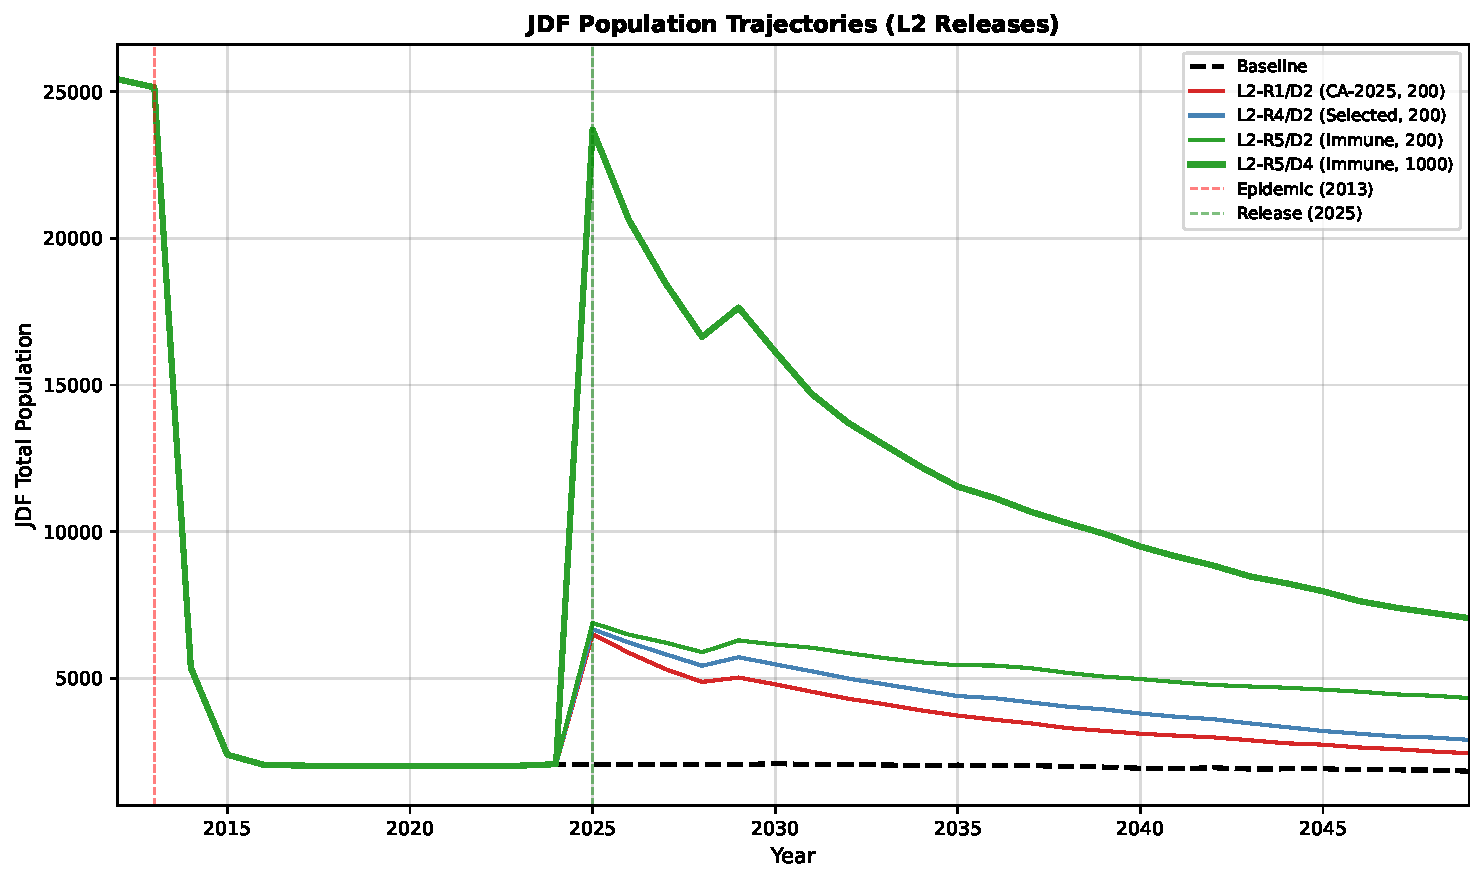
\includegraphics[width=\textwidth]{figures/fig_04_jdf_trajectories.pdf}
  \caption{\textbf{JDF population trajectories for L2 releases at selected R$\times$D combinations.} R5/D4 (immune, saturation) achieves the highest JDF recovery at 27.7\%, while R5/D2 reaches 17.0\%. Low-resistance stocks (R2, R3) at high density show declining JDF recovery---the competitive dilution effect is present but attenuated relative to California. The baseline (7.2\%) represents the trajectory without any intervention.}
  \label{fig:jdf_traj}
\end{figure}


% ── 3.5 Competitive Dilution ────────────────────────────────────
\subsection{Competitive Dilution: When More Is Less}
\label{sec:dilution}

\alertbox{Releasing low-resistance animals at high density is worse than doing nothing. This is the single most important finding for conservation policy.}

Figure~\ref{fig:dilution} presents the competitive dilution effect in its starkest form. For R1 ($\rbar=0.31$, CA-2025 survivors), CA-C recovery \emph{peaks} at D2 (200/site, 3.2\%) and then collapses: D3 drops to 1.8\%, and D4 crashes to 0.18\%---a 94\% reduction from D2. For R2 ($\rbar=0.15$, naive stock), the collapse is even more severe: D4 yields 0.03\%, a 98\% reduction from the D2 peak of 1.9\%.

The mechanism is straightforward but the implications are profound:
\begin{enumerate}[nosep]
  \item Released animals with low resistance ($\rbar \leq 0.31$) compete for space, food, and settlement substrate with resistant wild survivors.
  \item These released animals are highly susceptible to SSWD. Most die within years of release.
  \item Before dying, they have already consumed resources and occupied habitat, reducing the reproductive output and survival of resistant wild genotypes.
  \item Their offspring inherit low resistance, further diluting the resistance allele frequency in the population.
  \item At high release densities, this dilution overwhelms the natural selection that would otherwise favor resistant genotypes.
\end{enumerate}

At D4 (1000/site $=K$), the released animals numerically dominate the population at the moment of release, effectively resetting the allele frequency from whatever selection had achieved back toward the captive stock's $\rbar$. For R2 ($\rbar=0.15$), this is a regression to \emph{worse-than-pre-epidemic} vulnerability.

\begin{figure}[H]
  \centering
  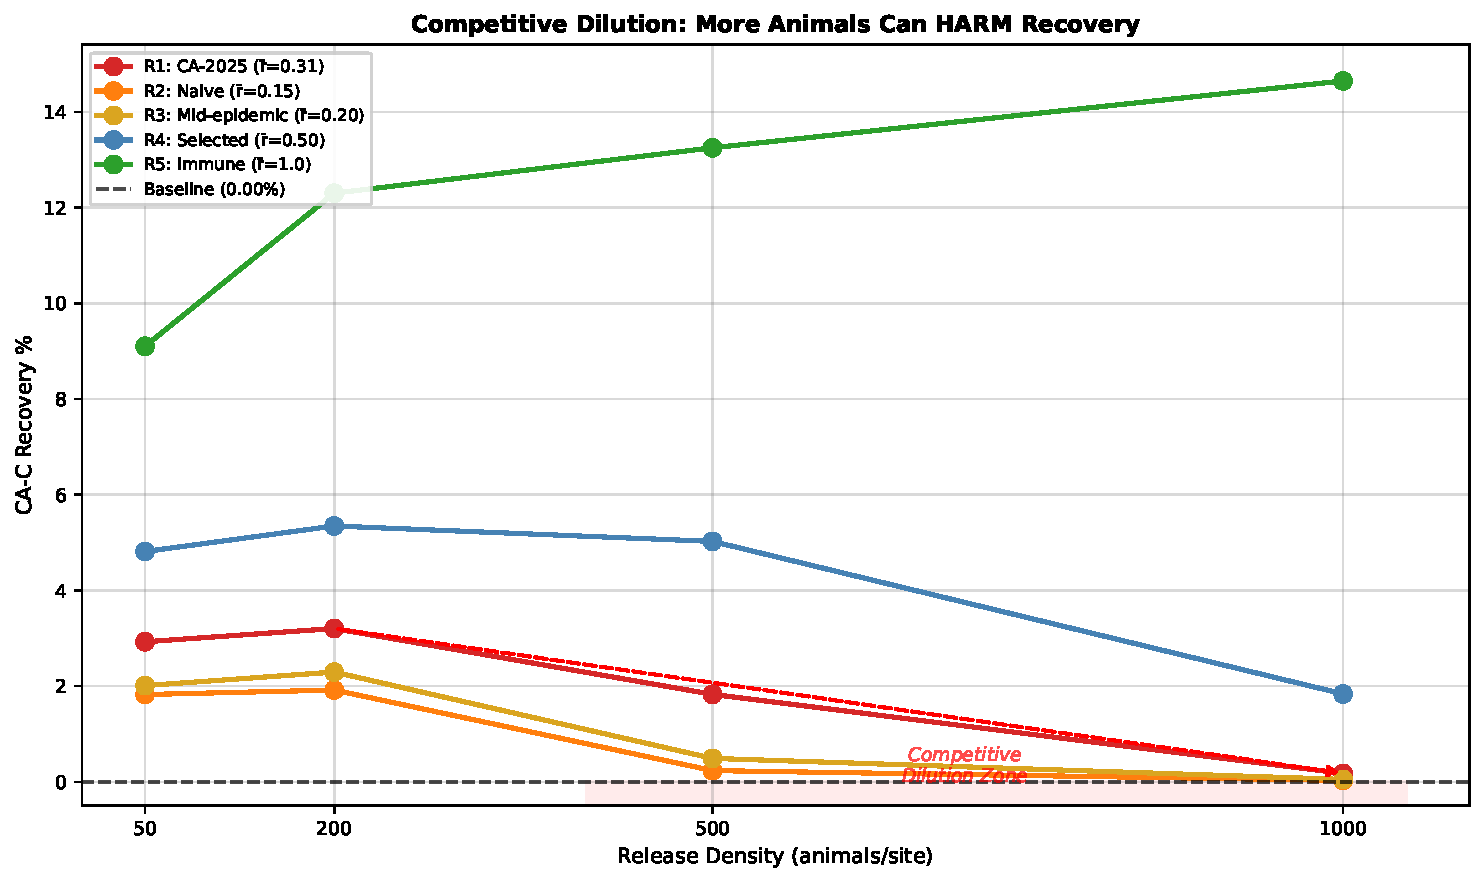
\includegraphics[width=\textwidth]{figures/fig_05_competitive_dilution.pdf}
  \caption{\textbf{Competitive dilution: CA-C recovery vs.\ release density for each resistance level (L1 scenarios).} For R1--R3, recovery \emph{declines} at high density---releasing more animals produces worse outcomes. R1/D4 (0.18\%) is worse than R1/D1 (2.93\%). R2/D4 (0.03\%) is functionally extinct. Only R5 shows a monotonically positive density--response. R4 shows a mild optimum near D2 before density effects begin to erode gains at D4 (1.8\%). The crossover between positive and negative density effects occurs at approximately $\rbar = 0.4$--$0.5$.}
  \label{fig:dilution}
\end{figure}


% ── 3.6 Resistance Threshold ────────────────────────────────────
\subsection{Resistance Threshold}

Figure~\ref{fig:threshold} shows CA-C recovery as a function of mean resistance ($\rbar$) at fixed D2 density (200/site). The relationship is strongly nonlinear: recovery is essentially flat at 2--3\% for $\rbar$ from 0.15 to 0.31, then begins to rise at $\rbar = 0.50$ (R4, 5.4\%), and accelerates dramatically to 12.3\% at $\rbar = 1.0$ (R5).

This threshold behavior implies that incremental improvements in resistance below $\rbar \approx 0.4$ produce negligible recovery gains---the disease simply kills susceptible animals faster than they can reproduce. Only above a critical resistance threshold does the population become self-sustaining. For policy, this means half-measures in breeding programs (e.g., using mid-epidemic stock at $\rbar=0.20$) will fail; the target must be aggressive selection toward $\rbar \geq 0.5$.

\begin{figure}[H]
  \centering
  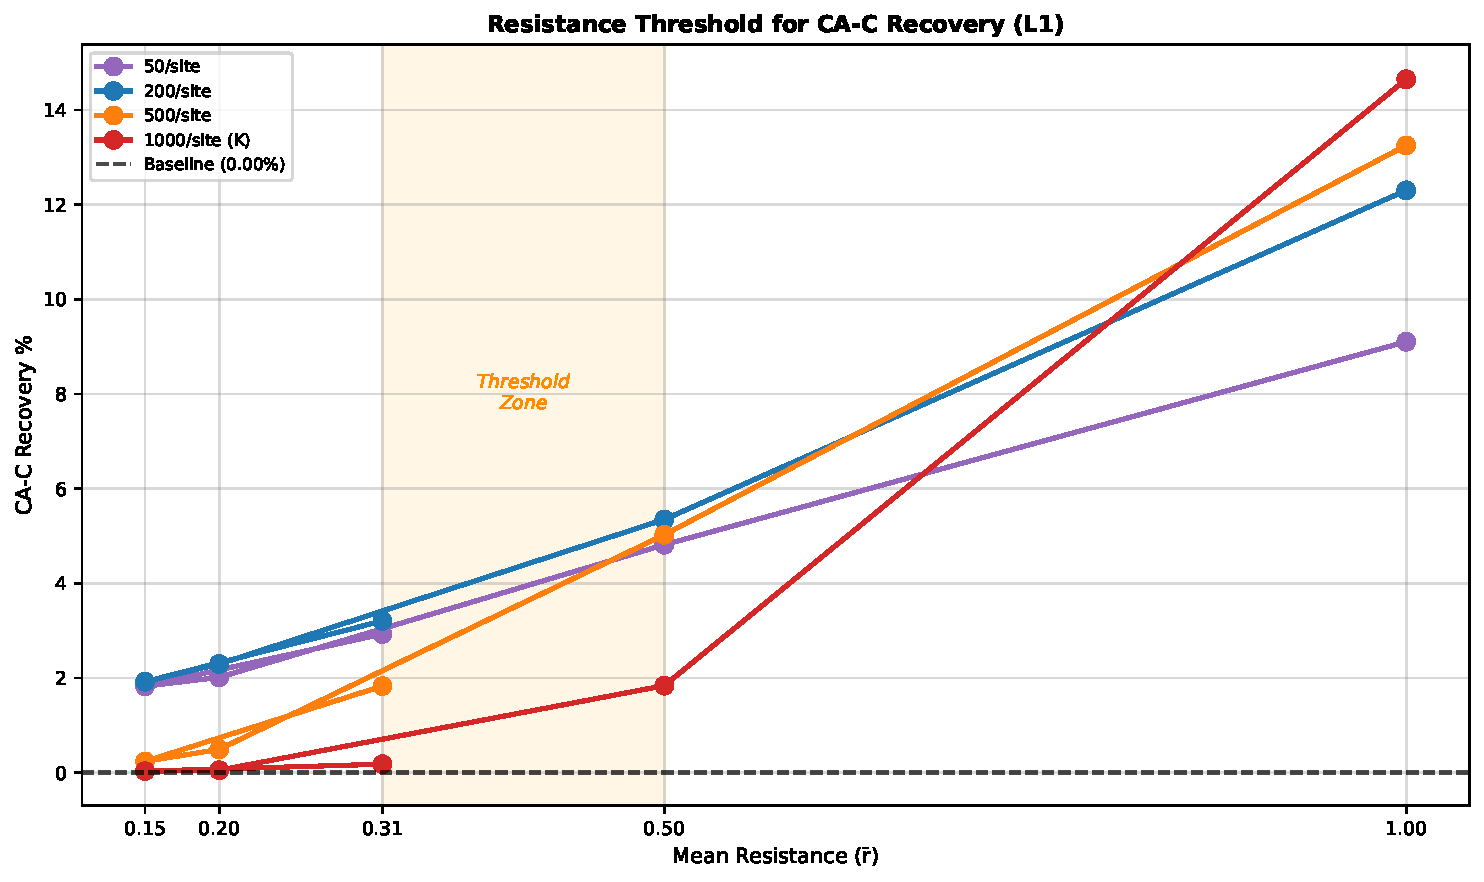
\includegraphics[width=\textwidth]{figures/fig_06_resistance_threshold.pdf}
  \caption{\textbf{Resistance threshold: CA-C recovery vs.\ mean resistance allele frequency at D2 (200/site).} The relationship is sharply nonlinear with a threshold near $\rbar \approx 0.4$. Below this threshold, recovery is marginal (1.9--3.2\%) regardless of $\rbar$. Above it, recovery scales steeply: R4 ($\rbar=0.50$) achieves 5.4\%, R5 ($\rbar=1.0$) reaches 12.3\%. This threshold defines the minimum breeding program target.}
  \label{fig:threshold}
\end{figure}


% ── 3.7 Dose-Response ───────────────────────────────────────────
\subsection{Dose-Response Curves}

Figure~\ref{fig:dose} expands the density dimension across all five resistance levels. R5 shows a clean positive dose-response across the full density range: 9.1\% (D1) $\rightarrow$ 12.3\% (D2) $\rightarrow$ 13.3\% (D3) $\rightarrow$ 14.6\% (D4) in CA-C. However, note the diminishing returns: the D1$\rightarrow$D2 step (4$\times$ animals) gains 3.2 pp, while D2$\rightarrow$D4 (5$\times$ animals) gains only 2.3 pp. This suggests that 200/site is near the efficient frontier for immune stock.

R4 ($\rbar=0.50$) shows a more complex response: positive through D2 (5.4\%), nearly flat at D3 (5.0\%), then declining at D4 (1.8\%). Even selected stock begins to suffer competitive dilution at saturation density. The critical observation is that \emph{even R4 is not fully safe from dilution at extreme density}.

\begin{figure}[H]
  \centering
  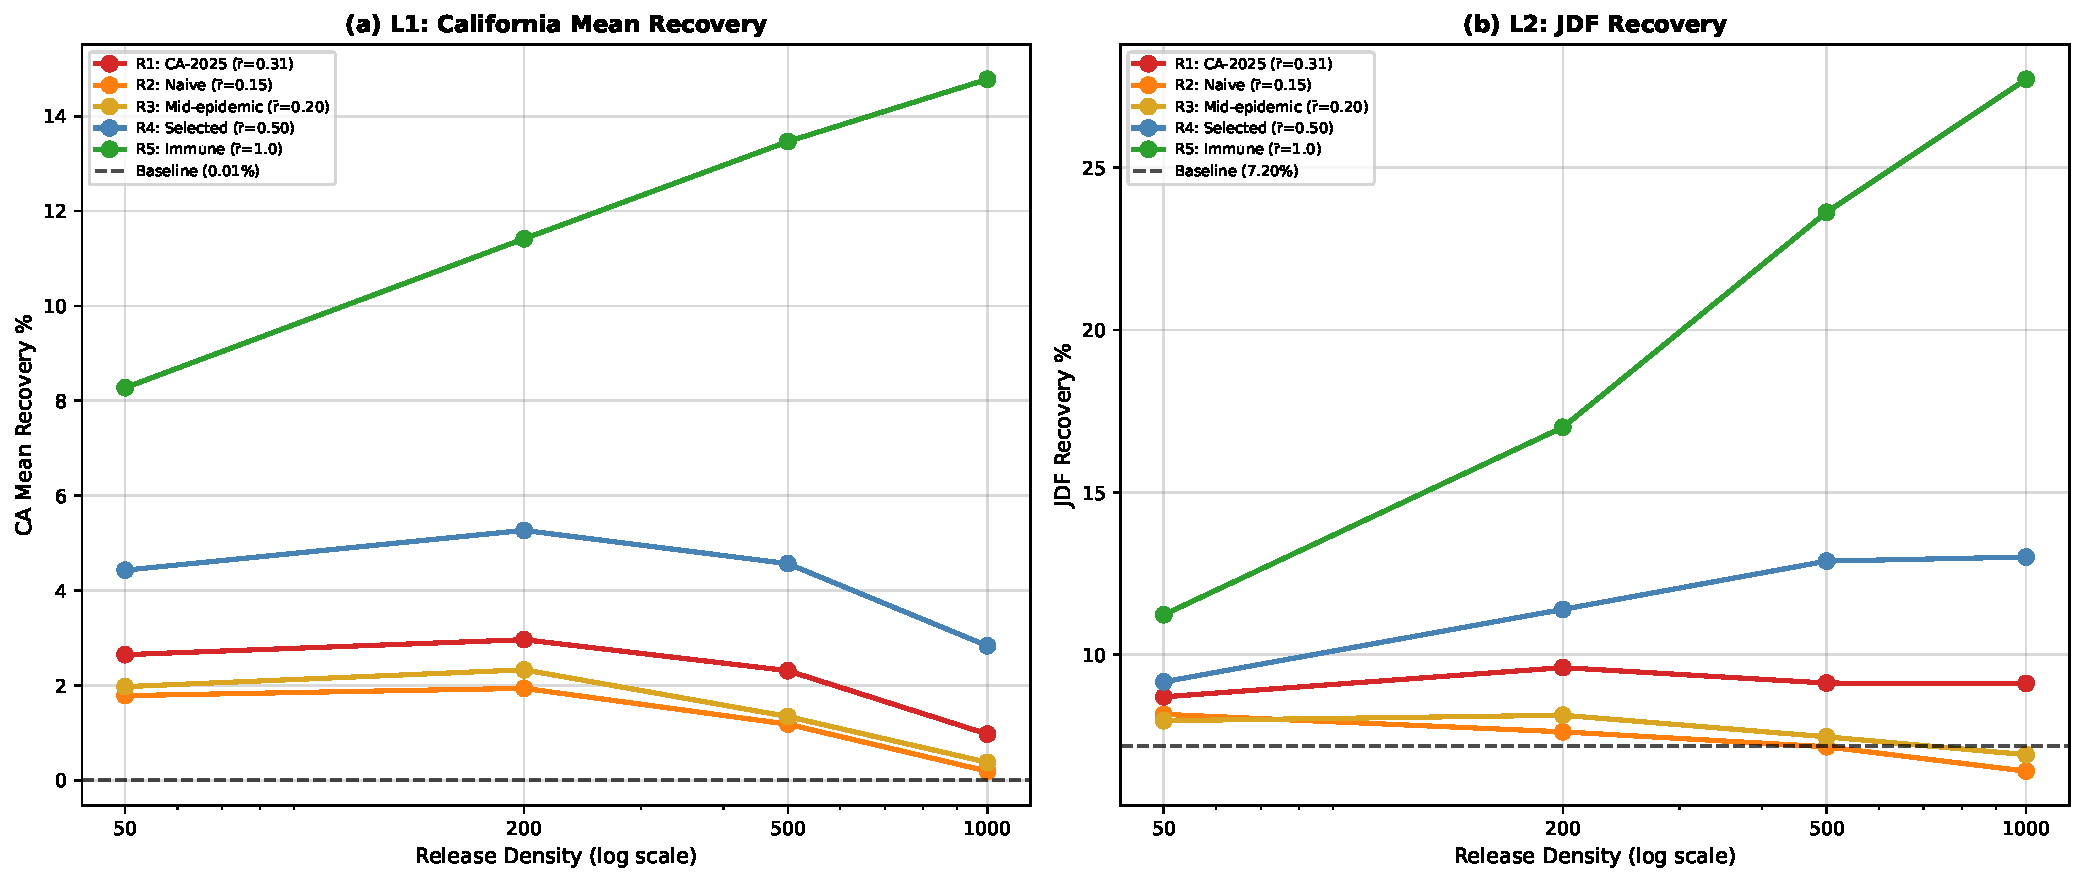
\includegraphics[width=\textwidth]{figures/fig_07_dose_response.pdf}
  \caption{\textbf{Dose-response curves: CA-C recovery vs.\ release density for all five resistance levels.} R5 (immune) shows positive but saturating dose-response. R4 (selected) peaks at D2--D3 then declines at D4. R1--R3 all show negative dose-response above D2, with R2 (naive) collapsing most severely. The optimal density depends critically on resistance level; prescribing a universal release density without knowing $\rbar$ is dangerous.}
  \label{fig:dose}
\end{figure}


% ── 3.8 Spillover ───────────────────────────────────────────────
\subsection{Spillover Assessment}

Figure~\ref{fig:spillover} maps regional spillover from each release location. L1 (Monterey) releases produce northward spillover into Oregon (OR: 0.75\% baseline $\rightarrow$ 3.7\% at R5/D4) and minor uplift in WA-O (3.2\% $\rightarrow$ 3.6\%), but no meaningful effect beyond the Strait of Juan de Fuca. Southward spillover into CA-S is present: 0.0\% baseline $\rightarrow$ 8.4\% at R5/D4 for CA-S, indicating that Monterey releases can seed the Southern California Bight via southward larval transport.

L2 (Friday Harbor) releases enhance JDF strongly (7.2\% $\rightarrow$ 27.7\% at R5/D4) with modest spillover to surrounding Salish Sea regions, but \emph{zero} spillover to any California region. The oceanographic barrier between the Pacific Northwest and California is absolute in this model's connectivity matrix.

\begin{figure}[H]
  \centering
  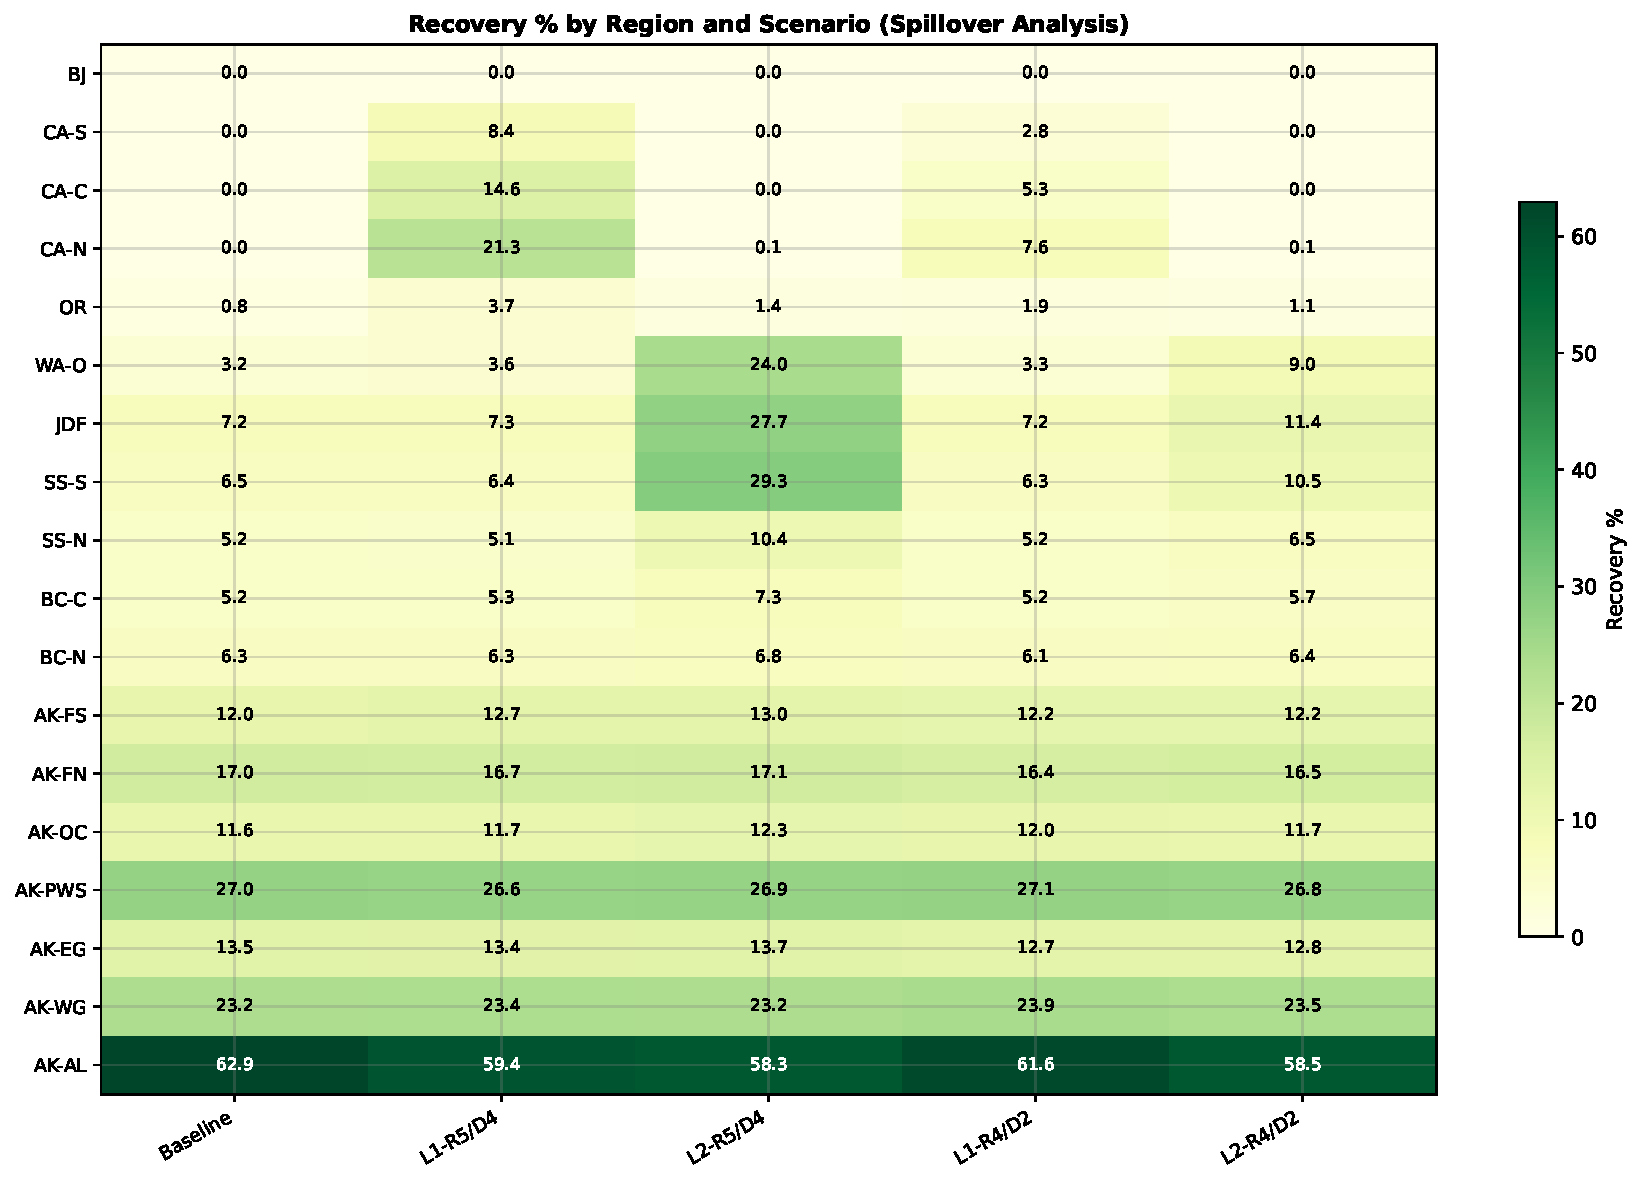
\includegraphics[width=\textwidth]{figures/fig_08_spillover_heatmap.pdf}
  \caption{\textbf{Spillover heatmap: recovery change from baseline across all 18 regions for selected scenarios.} L1 (Monterey) releases propagate through CA-S, CA-C, CA-N, and weakly into OR. L2 (Friday Harbor) releases propagate through JDF and adjacent Salish Sea regions only. The WA--CA gap is an absolute barrier to southward larval transport. Northern regions (BC-N, AK) are invariant to either release location.}
  \label{fig:spillover}
\end{figure}


% ── 3.9 Alaska Stability ────────────────────────────────────────
\subsection{Alaska Stability}

Figure~\ref{fig:ak} overlays all 40 AK-PWS trajectories. The spread is negligible: 26.2--27.8\% final recovery across every scenario, baseline included. Alaska's populations are driven entirely by local dynamics---temperature regime, endemic disease pressure, and intrinsic growth---and are not influenced by reintroduction events $>$3000\,km to the south.

This confirms that AK-PWS functions as a self-sustaining refugium. Conservation resources directed at Alaska would be redundant; the population is stable without intervention. Conversely, Alaska cannot serve as a source population for California recovery, as the larval dispersal kernel does not connect these regions on ecologically relevant timescales.

\begin{figure}[H]
  \centering
  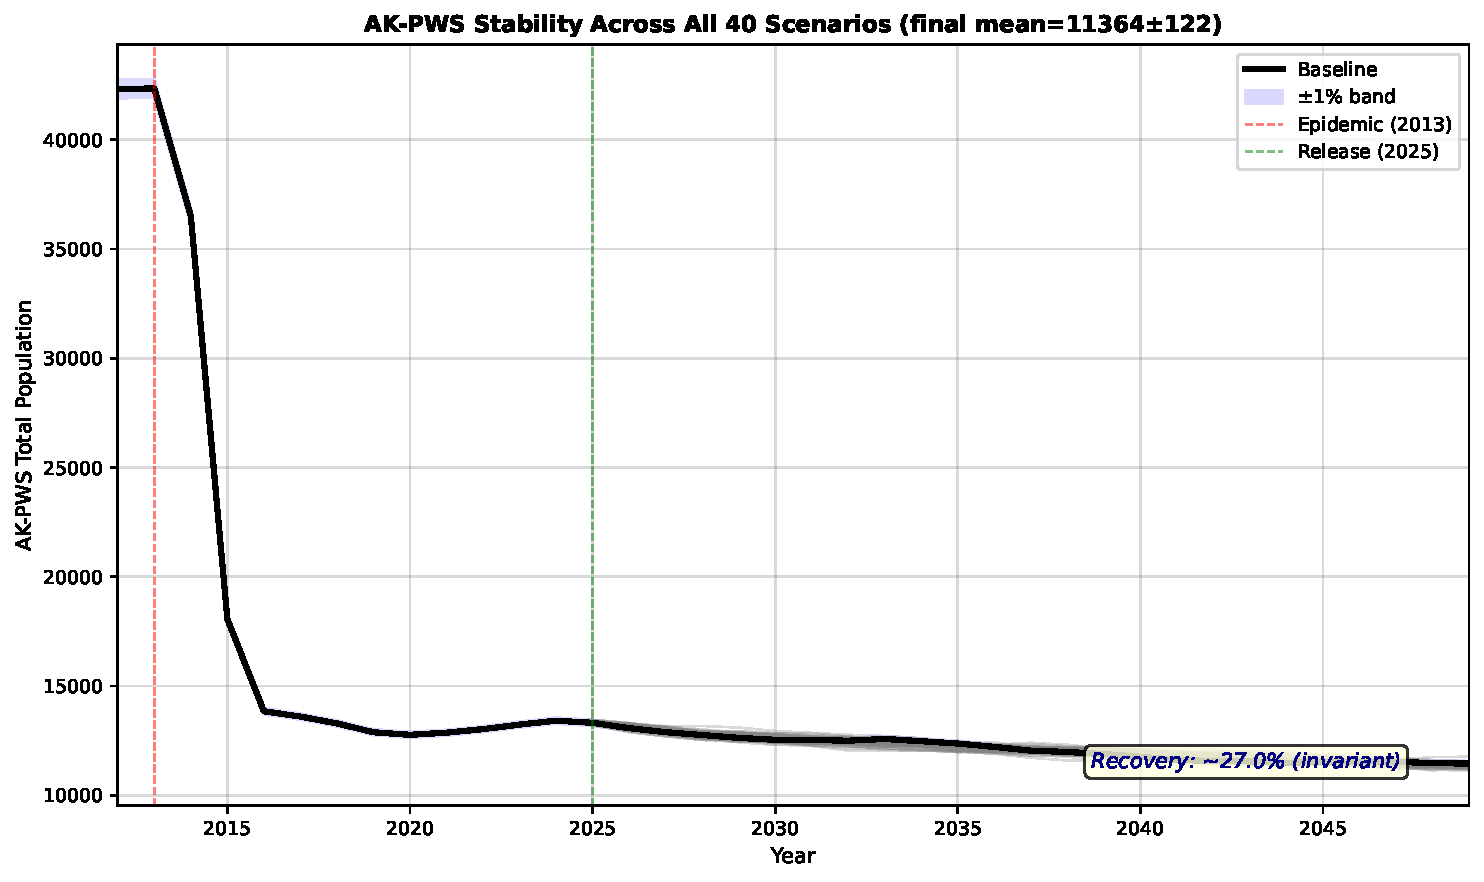
\includegraphics[width=\textwidth]{figures/fig_09_ak_stability.pdf}
  \caption{\textbf{AK-PWS population trajectories across all 40 reintroduction scenarios (gray) and baseline (black).} All trajectories converge to 26.2--27.8\% by 2050. The near-total overlap demonstrates that Alaskan populations are decoupled from lower-latitude dynamics and insensitive to any reintroduction intervention. AK-PWS is a self-sustaining refugium requiring no conservation action.}
  \label{fig:ak}
\end{figure}


% ── 3.10 Regional Map ───────────────────────────────────────────
\subsection{Regional Recovery Map}

Figure~\ref{fig:map} presents a geographic view of regional recovery under the best-case scenario (L1/R5/D4) compared to baseline. The map highlights the stark latitudinal gradient: California regions show the largest absolute improvement (from 0\% to 8--21\%), Oregon shows modest gains (0.8\% $\rightarrow$ 3.7\%), and everything north of Juan de Fuca is unchanged.

The geographic pattern reinforces two points: (1) California recovery requires California releases---there is no long-distance rescue; and (2) the improvement is geographically concentrated near the release site, with a north--south gradient reflecting the model's larval dispersal kernel.

\begin{figure}[H]
  \centering
  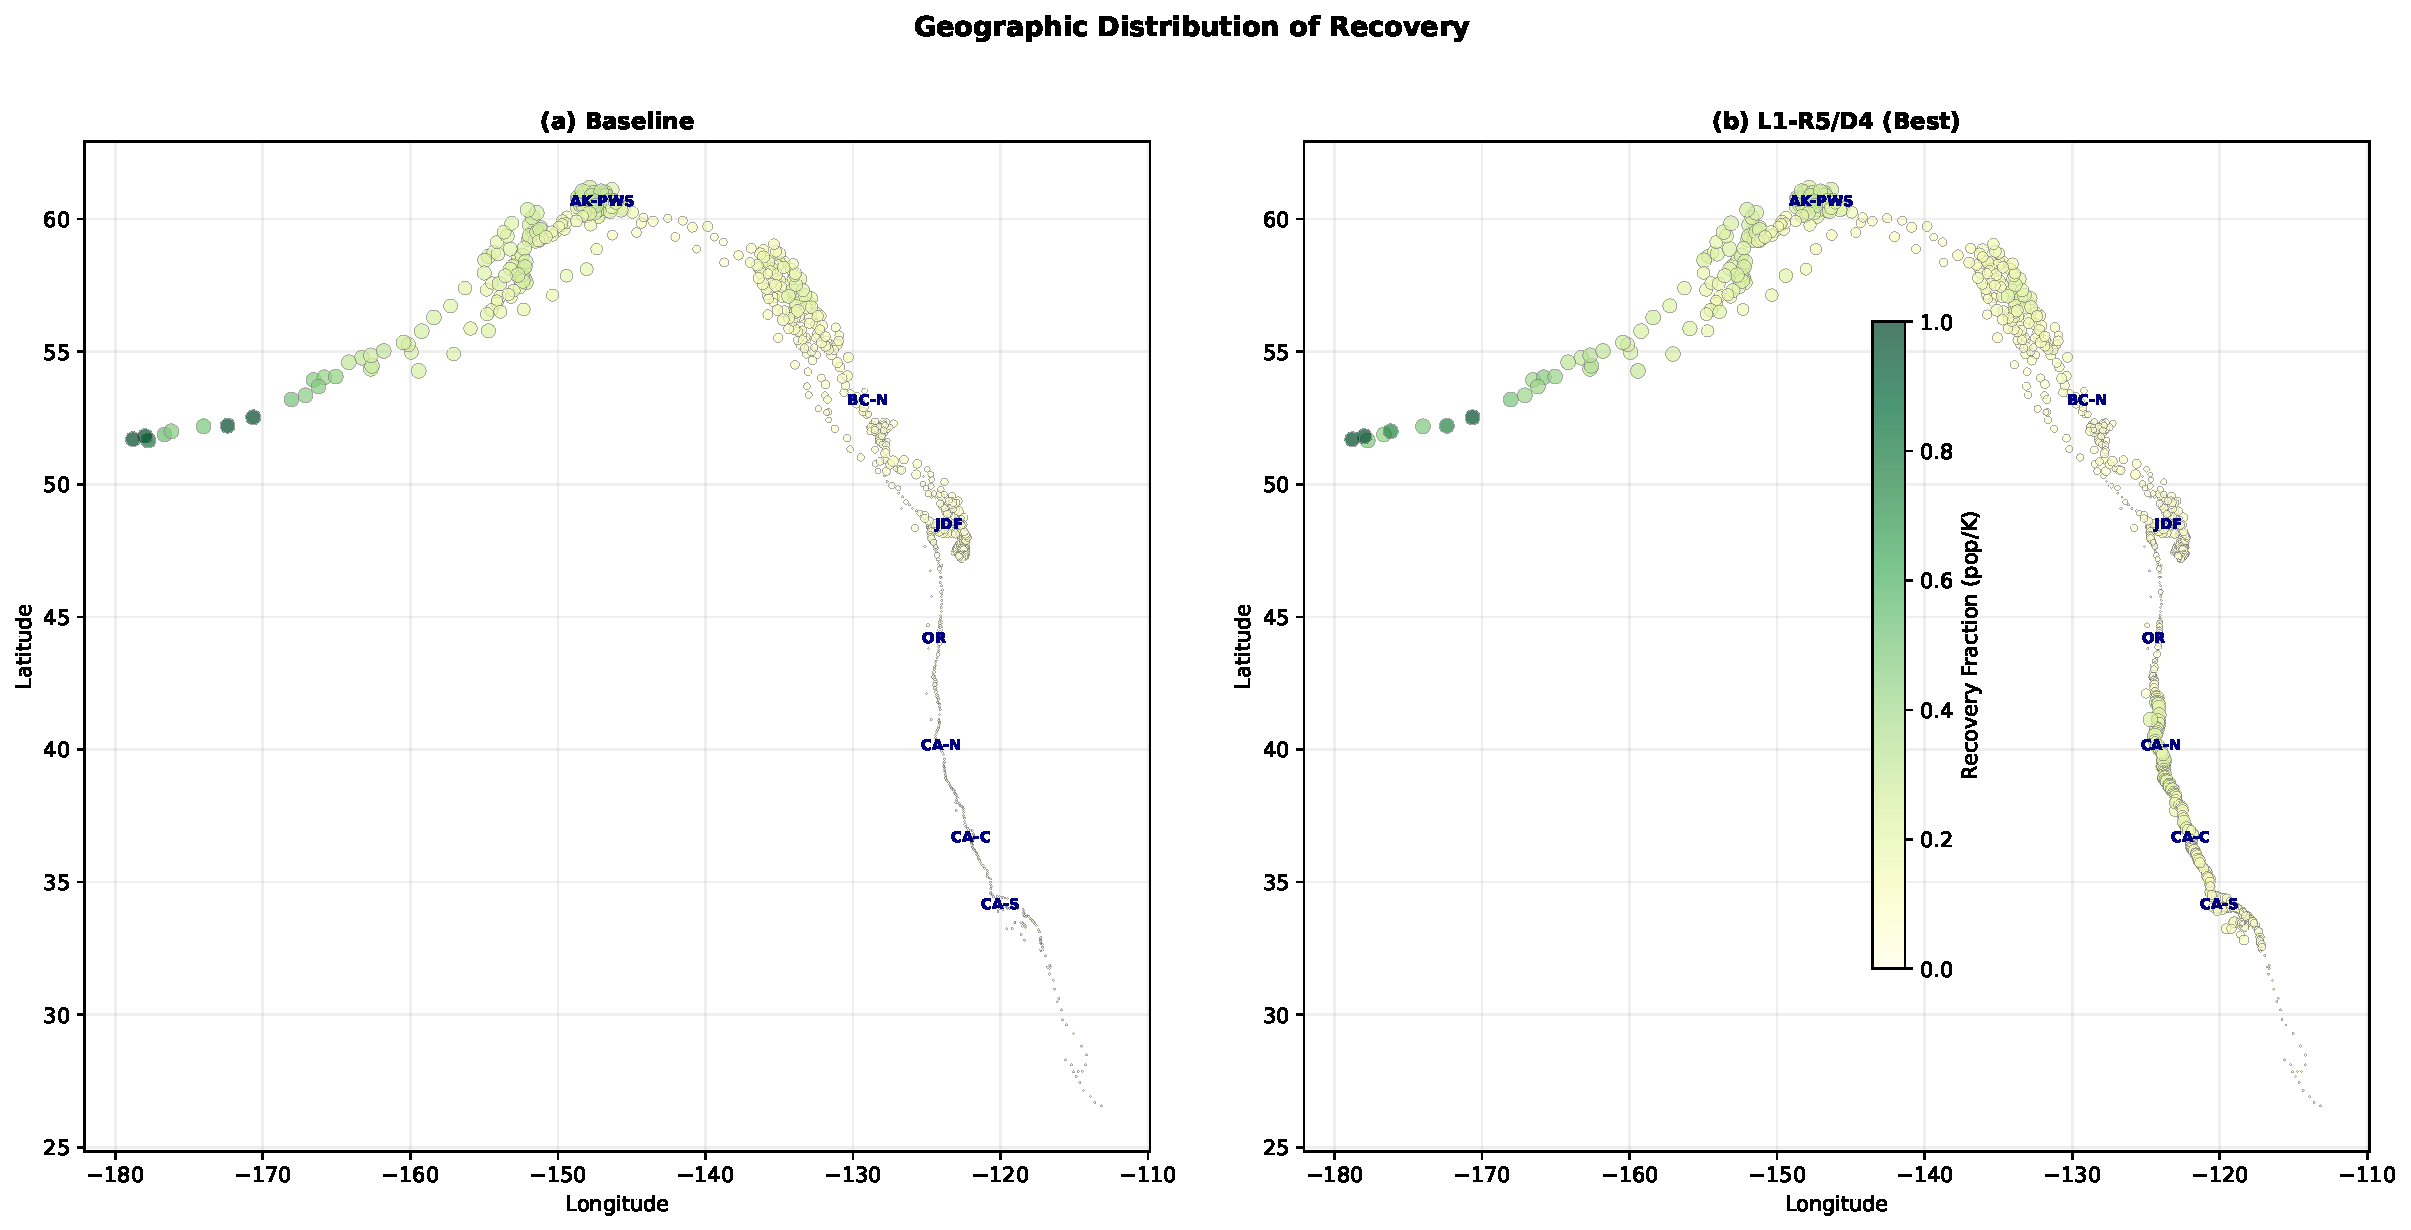
\includegraphics[width=\textwidth]{figures/fig_10_regional_map.pdf}
  \caption{\textbf{Geographic distribution of recovery: baseline (left) vs.\ best L1 scenario R5/D4 (right).} Circle size/color indicates recovery percentage by region. California transitions from empty (0\%) to partially recovered (8--21\%). Oregon shows modest improvement. All regions north of JDF are unchanged. The spatial footprint of reintroduction is limited to ${\sim}$1500\,km from the release site.}
  \label{fig:map}
\end{figure}


% ── 3.11 Interaction Plot ────────────────────────────────────────
\subsection{Genetics $\times$ Density Interaction}

Figure~\ref{fig:interaction} presents the full genetics $\times$ density interaction for CA recovery. The interaction is strongly disordinal: the effect of density \emph{reverses sign} depending on resistance level. For R5, density is beneficial (positive slope); for R1--R3, density is harmful (negative slope); R4 sits near the crossover.

This disordinal interaction means there is no single ``optimal density'' recommendation that applies across resistance levels. Policy prescriptions \emph{must} be conditional on the genetics of the release stock. A recommendation to ``release as many as possible'' would be catastrophic if applied to R2 stock but beneficial if applied to R5 stock.

\begin{figure}[H]
  \centering
  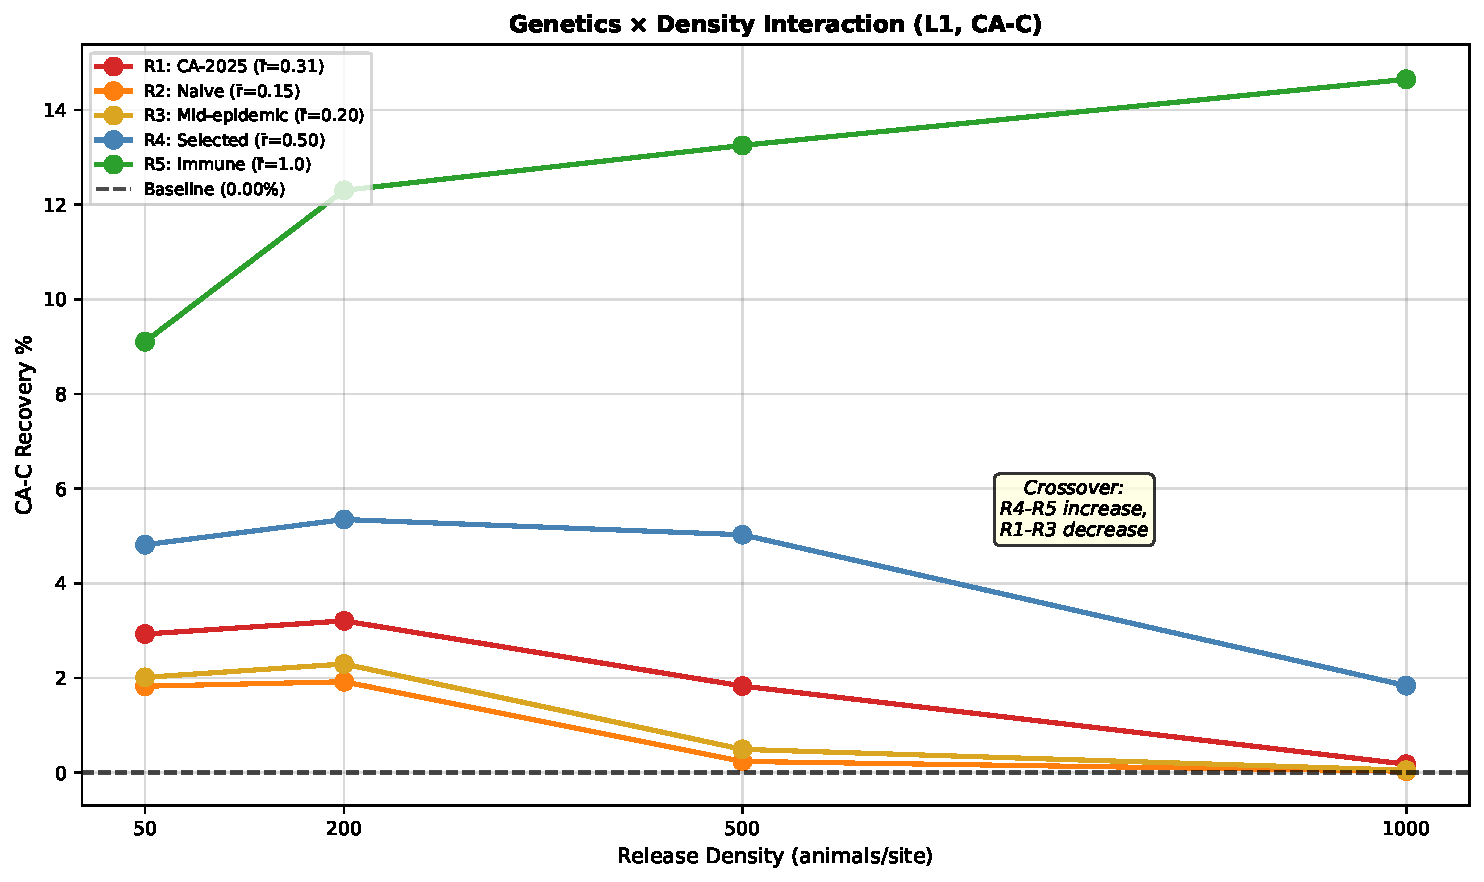
\includegraphics[width=\textwidth]{figures/fig_11_interaction_plot.pdf}
  \caption{\textbf{Genetics $\times$ density interaction plot for CA-C recovery.} Lines connect density levels within each resistance group. The crossing pattern is a textbook disordinal interaction: density helps high-resistance stock but harms low-resistance stock. The crossover occurs near $\rbar \approx 0.4$--$0.5$, defining the threshold above which ``release more'' is good advice.}
  \label{fig:interaction}
\end{figure}


% ── 3.12 CA Region Comparison ────────────────────────────────────
\subsection{California Sub-Regional Comparison}

Figure~\ref{fig:ca_regions} breaks down the California recovery by sub-region (CA-S, CA-C, CA-N) for L1 scenarios. A consistent north--south gradient emerges: CA-N recovers best (21.3\% at R5/D4), CA-C intermediate (14.6\%), and CA-S least (8.4\%). This gradient likely reflects the proximity to Northern California's more favorable thermal regime and connectivity to Oregon populations.

For R4, the pattern is similar but compressed: CA-N\,=\,7.6\%, CA-C\,=\,5.4\%, CA-S\,=\,2.8\% at D2. At D4, R4 shows dramatic collapse in CA-S (0.04\%) and CA-C (1.8\%), while CA-N partially holds at 6.6\%---suggesting that northern sub-regions are more resilient to competitive dilution, possibly due to higher larval connectivity to the Oregon population which acts as a buffer.

\begin{figure}[H]
  \centering
  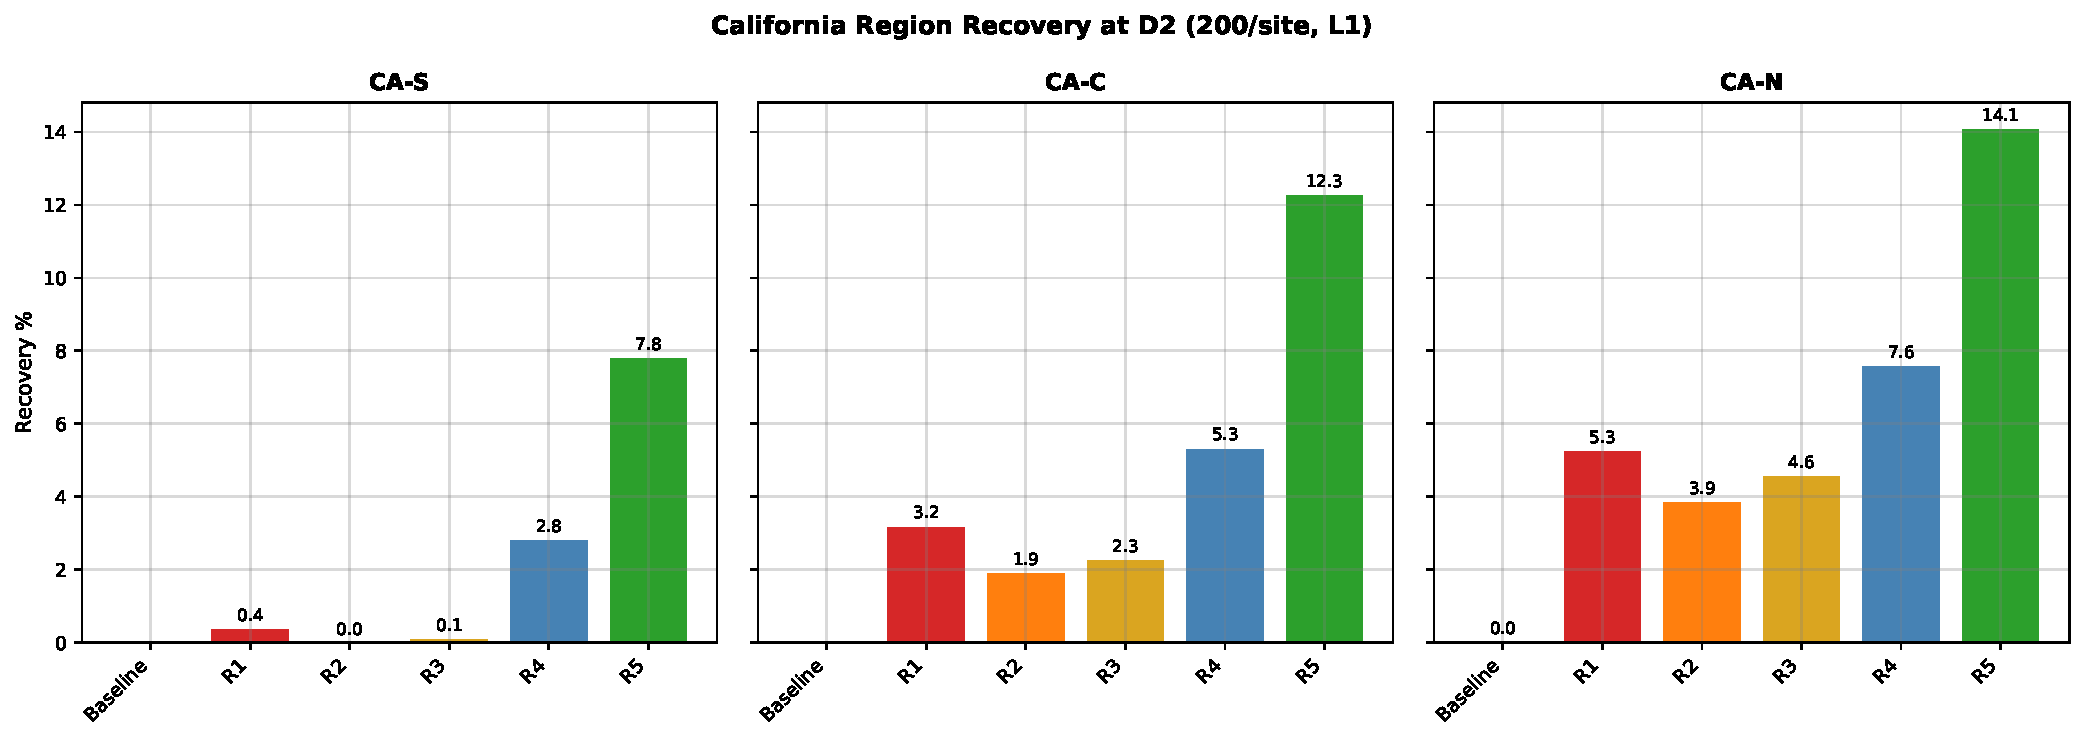
\includegraphics[width=\textwidth]{figures/fig_12_ca_region_comparison.pdf}
  \caption{\textbf{California sub-regional recovery across L1 scenarios.} CA-N consistently outperforms CA-C and CA-S across all genetics$\times$density combinations. The north--south gradient reflects proximity to the resistant Oregon population and more favorable thermal conditions. At R5/D4: CA-N\,=\,21.3\%, CA-C\,=\,14.6\%, CA-S\,=\,8.4\%. The competitive dilution effect is most severe in CA-S, which collapses to 0\% for R1--R3 at D3--D4.}
  \label{fig:ca_regions}
\end{figure}


% ── 3.13 Genetics Evolution ─────────────────────────────────────
\subsection{Resistance Allele Dynamics}

Figure~\ref{fig:genetics} tracks the evolution of resistance allele frequency in the CA-C population over time for selected scenarios. In the baseline, $\rbar$ drifts upward slowly through natural selection (survivors are disproportionately resistant), but the population is too small for this to matter ecologically.

When low-resistance stock is released at high density (R2/D4), $\rbar$ is immediately diluted at the release point, dropping sharply. This genetic dilution persists for years because the large number of susceptible animals and their offspring overwhelm the resistant fraction. The population never recovers because SSWD mortality prevents the re-evolution of resistance on the timescale of the simulation.

In contrast, R5/D4 maintains $\rbar$ at or near 1.0 post-release, and the population grows monotonically because disease mortality is negligible.

\begin{figure}[H]
  \centering
  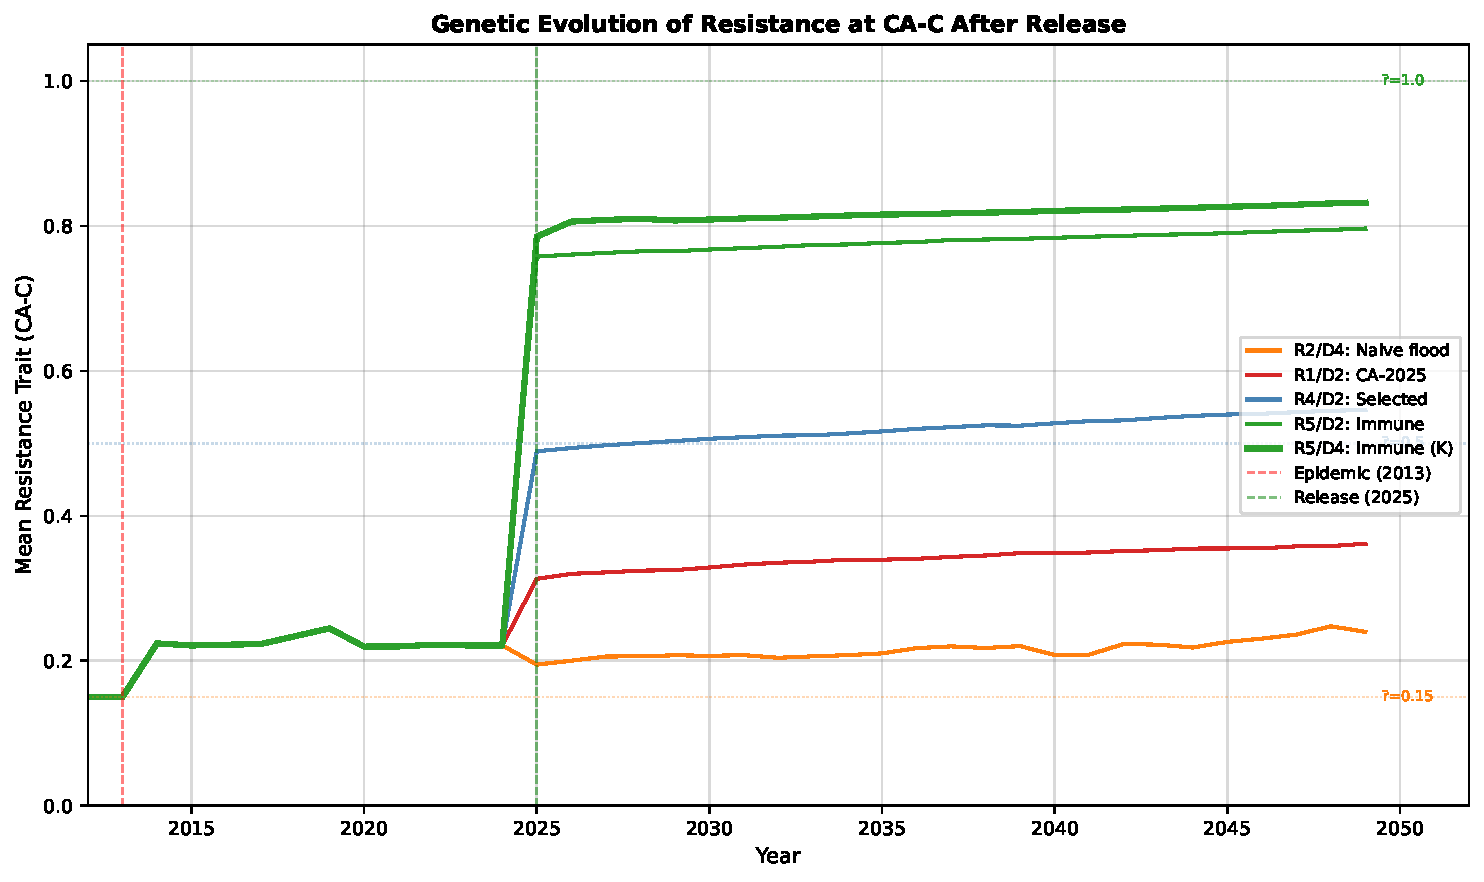
\includegraphics[width=\textwidth]{figures/fig_13_genetics_evolution.pdf}
  \caption{\textbf{Resistance allele dynamics in the CA-C population.} For R2/D4 (naive stock at saturation density), the mean resistance drops sharply at release and never recovers---the genetic dilution is permanent on the 25-year timescale. R1/D4 shows a similar but less severe dilution. R5 maintains high resistance throughout, enabling sustained population growth. The genetic mechanism underlies the competitive dilution phenomenon: it is fundamentally a problem of allele frequency, not population size.}
  \label{fig:genetics}
\end{figure}


% ── 3.14 Summary Table ──────────────────────────────────────────
\subsection{Full Results Summary}

Figure~\ref{fig:summary} presents the complete results table for all 40 scenarios plus baseline. Key metrics include final population fraction, regional recovery percentages, and the relative change from baseline for each focal region.

\begin{figure}[H]
  \centering
  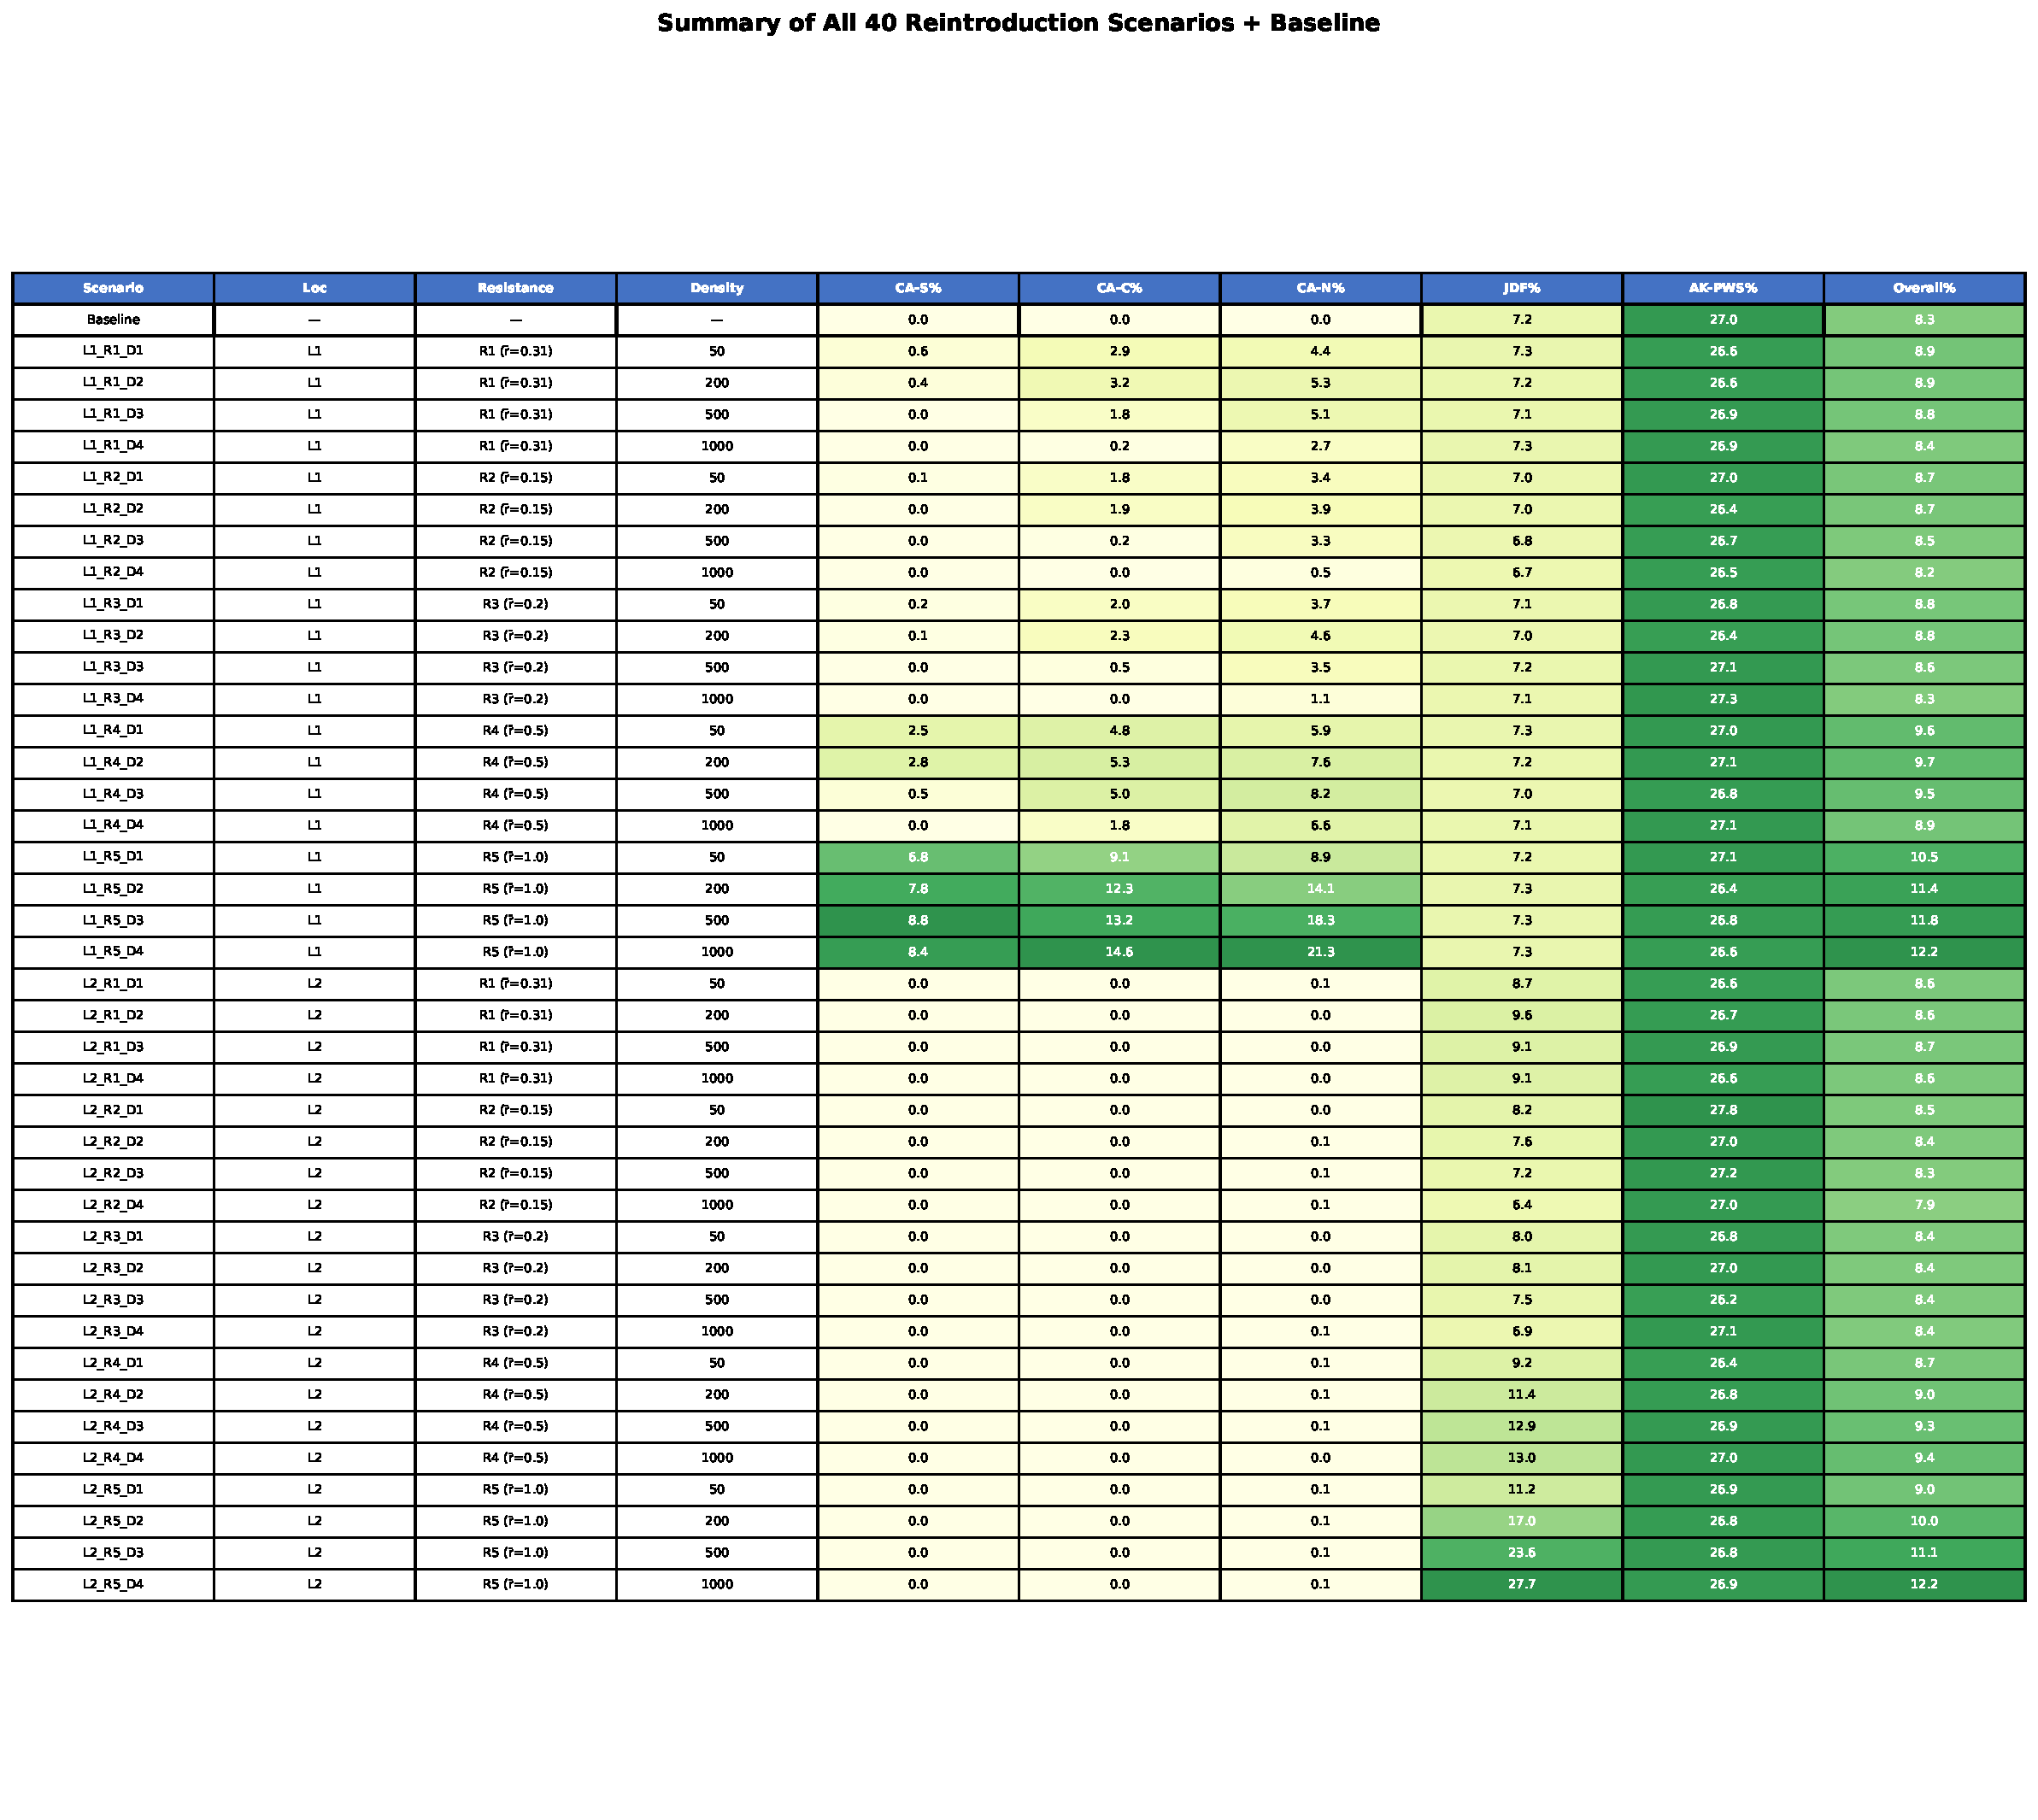
\includegraphics[width=\textwidth]{figures/fig_14_summary_table.pdf}
  \caption{\textbf{Summary table of all 40 scenarios and baseline.} Each row is one scenario (Location $\times$ Resistance $\times$ Density), with columns for final recovery in each focal region (CA-S, CA-C, CA-N, JDF, AK-PWS) and total metapopulation. Cells are color-coded by recovery level. The competitive dilution pattern is visible in the declining CA columns for R1--R3 as density increases. L2 scenarios show CA columns locked at 0\%.}
  \label{fig:summary}
\end{figure}


% ══════════════════════════════════════════════════════════════════
\section{Discussion}
% ══════════════════════════════════════════════════════════════════

\subsection{Conservation Implications of Competitive Dilution}

The competitive dilution finding challenges the prevailing assumption that ``more animals = better recovery'' for reintroduction programs. In disease-impacted systems where host resistance is heritable and under active selection, the genetic quality of released stock is more important than the quantity. This is not merely a theoretical concern---the model shows that releasing 1000/site of naive stock \emph{actively extirpates} populations that would otherwise persist at low levels.

The mechanism operates through three reinforcing pathways:

\begin{enumerate}[nosep]
  \item \textbf{Direct resource competition.} Released animals consume food and occupy habitat, reducing per-capita resources for resistant wild survivors. At $D4 = K$, released animals fill the site to carrying capacity, leaving zero headroom for wild individuals.
  \item \textbf{Genetic swamping.} Released animals interbreed with wild survivors, producing offspring with intermediate resistance. If the captive stock has low $\rbar$, this reduces the mean resistance of the next generation.
  \item \textbf{Disease amplification.} Susceptible released animals become infected and serve as disease reservoirs, increasing local pathogen pressure on all individuals---including resistant ones whose survival probability, while higher, is not absolute at $\rbar < 1.0$.
\end{enumerate}

These three pathways compound: more released animals means more competition, more genetic dilution, \emph{and} more disease amplification, creating a triple negative feedback that overwhelms any numerical benefit of the release.

The general conditions under which competitive dilution occurs are:
\begin{enumerate}[nosep]
  \item An endemic pathogen imposes strong selection for resistance
  \item Wild survivors have undergone natural selection (elevated $\rbar$)
  \item Captive stock has lower resistance than wild survivors
  \item Released animals compete directly with wild individuals for limiting resources
  \item Release density is high enough to shift allele frequencies at the population level
\end{enumerate}

These conditions are not unique to \textit{Pycnopodia}. Amphibian reintroduction programs facing \textit{Batrachochytrium dendrobatidis} (Bd chytrid), coral restoration in the face of white-band and stony coral tissue loss disease, and even ungulate translocations in systems with chronic wasting disease (CWD) should consider the competitive dilution risk. The principle generalizes: \textbf{in any system with an endemic pathogen and heritable resistance, releasing genetically inferior stock can be worse than doing nothing.}

\subsection{Interpreting the Resistance Threshold}

The nonlinear relationship between $\rbar$ and recovery (Section~\ref{sec:dilution}, Figure~\ref{fig:threshold}) has a mechanistic interpretation rooted in the basic reproductive number of the disease. At low $\rbar$, most individuals are susceptible and disease-induced mortality exceeds the population's reproductive capacity---the population cannot grow because new recruits die faster than they are born. Above a critical $\rbar$, sufficient individuals survive infection to maintain positive population growth, and the population enters a recovery trajectory.

This threshold is analogous to the concept of herd immunity in epidemiology: when a sufficient fraction of the population is resistant, transmission chains break and the pathogen can no longer suppress population growth. For SSWD in the California thermal environment, our results place this threshold near $\rbar \approx 0.4$--$0.5$.

The practical implication is sobering: incremental improvements in captive stock resistance (e.g., from $\rbar = 0.15$ to $\rbar = 0.20$) produce \emph{no detectable population benefit}. The breeding program must achieve a step-change in resistance to cross the threshold. This argues against gradual, conservative breeding approaches and in favor of aggressive selection intensity, potentially including marker-assisted selection or genomic prediction if suitable genetic markers can be identified.

\subsection{The Larval Transport Barrier}

The complete absence of California benefit from Washington releases deserves attention. The oceanographic connectivity matrix shows that dominant current flow in the Northeast Pacific is northward along the coast (the Alaska Current / North Pacific Current system). Southward larval transport occurs primarily within the California Current, which does not extend into the Puget Sound / Juan de Fuca system.

This means that a reintroduction program centered on Friday Harbor, WA---while beneficial for local JDF populations---cannot serve as a ``seed source'' for California recovery. The two regions are effectively isolated on the timescale of larval dispersal (weeks), and adult migration in \textit{Pycnopodia} is too slow to bridge the $>$1500\,km gap on decadal timescales.

The corollary is that California populations must be self-seeding. Any recovery in CA depends on local reproduction by resistant individuals, not immigration from northern populations. This reinforces the urgency of California-focused releases with high-resistance stock.

\subsection{Breeding Program Recommendations}

The results strongly support prioritizing resistance selection over rapid population expansion in captive breeding:

\begin{enumerate}[nosep]
  \item \textbf{Target $\rbar \geq 0.5$ before large-scale release.} The resistance threshold (Section~3.6) shows negligible recovery gains below this value. Breeding programs should invest in challenge assays and genomic selection to push $\rbar$ above 0.5 within 3--5 generations.
  
  \item \textbf{Use moderate release densities (200/site) even for high-resistance stock.} Diminishing returns above D2 mean that distributing animals across more sites is more efficient than saturating fewer sites.
  
  \item \textbf{Release in California, not Washington.} The absence of southward larval transport means WA releases contribute nothing to CA recovery. If the goal is California population restoration, releases must occur within the California Current system.
  
  \item \textbf{Monitor resistance allele frequency post-release.} If genetic tools are available, tracking $\rbar$ in the wild population post-release would provide early warning of dilution effects before population-level consequences become apparent.
\end{enumerate}

\subsection{Limitations}

Several caveats apply:
\begin{itemize}[nosep]
  \item The model uses a single stochastic seed (42). While results are internally consistent, confidence intervals would require ensemble runs.
  \item Resistance is modeled as a single heritable trait. Real SSWD resistance likely involves multiple loci with epistatic interactions.
  \item The connectivity matrix is static. Climate-driven changes in ocean circulation could alter larval transport pathways by 2050.
  \item Environmental stochasticity (marine heatwaves, prey availability) is simplified. Real populations will experience additional variance.
  \item The $\rbar=1.0$ (R5) scenario is aspirational. Whether full immunity can be achieved through selective breeding is unknown.
\end{itemize}

\subsection{The BC-N Puzzle}

BC-N (Northern British Columbia) recovers to ${\sim}$6\% in all 40 scenarios and the baseline, with a range of only 5.8--6.8\%. Neither California nor Washington releases influence this region. BC-N appears to be in a stable low-density equilibrium maintained by local disease dynamics and moderate thermal stress, disconnected from both the California reintroduction effect and the Alaskan refugium. Understanding BC-N's stagnation would require targeted investigation of its local connectivity, disease pressure, and thermal regime.


% ══════════════════════════════════════════════════════════════════
\section{Conclusions}
% ══════════════════════════════════════════════════════════════════

Based on 40 full-factorial reintroduction scenarios spanning five resistance profiles, four release densities, and two release locations, we reach the following actionable conclusions:

\begin{enumerate}[leftmargin=2em]
  \item \textbf{Breed for resistance, not numbers.} Only stock with $\rbar \geq 0.5$ (ideally approaching 1.0) should be released at scale. Below this threshold, reintroduction is ineffective; at high density with low $\rbar$, it is actively harmful through competitive dilution of resistance alleles.
  
  \item \textbf{Release in California, at moderate density.} California populations cannot be rescued from Washington. All releases targeting CA recovery must occur within the California Current system. A release density of ${\sim}$200/site represents the efficient frontier, balancing recovery gains against diminishing returns and dilution risk.
  
  \item \textbf{Do not intervene in Alaska.} AK-PWS is self-sustaining at 27\% of pre-epidemic levels and insensitive to any intervention tested. Conservation resources are better allocated to California breeding programs.
  
  \item \textbf{Treat competitive dilution as a first-order risk.} Any reintroduction program must include resistance screening of release stock and genetic monitoring of wild populations post-release. The default assumption should be that releasing unscreened animals at high density will cause harm.
  
  \item \textbf{Invest in resistance genomics.} The difference between R4 ($\rbar=0.50$, moderate recovery) and R5 ($\rbar=1.0$, strong recovery) represents the gap between current selective breeding capability and what is needed. Genomic tools to accelerate resistance selection---marker-assisted selection, genomic prediction, or even gene editing---should be prioritized.
\end{enumerate}

\clearpage
% ══════════════════════════════════════════════════════════════════
\appendix
\section{Full Scenario Results}
% ══════════════════════════════════════════════════════════════════

Table~\ref{tab:full_results} presents recovery percentages for all 40 scenarios and the baseline across the five focal regions: CA-S, CA-C, CA-N, JDF, and AK-PWS. Values represent the final population in 2050 as a percentage of the pre-epidemic reference population ($K_\text{ref}=5000$).

\begin{small}
\begin{longtable}{llrrrrrr}
\caption{Full results for all 40 reintroduction scenarios and baseline. Recovery is reported as percentage of pre-epidemic reference population by region. \textbf{Bold} values indicate improvement $>$5\% over baseline; \textcolor{alertred}{red} values indicate competitive dilution (worse than the same genetics at lower density).}
\label{tab:full_results} \\
\toprule
\textbf{Scenario} & $\rbar$ & \textbf{D} & \textbf{CA-S} & \textbf{CA-C} & \textbf{CA-N} & \textbf{JDF} & \textbf{AK-PWS} \\
\midrule
\endfirsthead
\multicolumn{8}{c}{\small\itshape (continued from previous page)} \\
\toprule
\textbf{Scenario} & $\rbar$ & \textbf{D} & \textbf{CA-S} & \textbf{CA-C} & \textbf{CA-N} & \textbf{JDF} & \textbf{AK-PWS} \\
\midrule
\endhead
\midrule
\multicolumn{8}{r}{\small\itshape (continued on next page)} \\
\endfoot
\bottomrule
\endlastfoot
% Baseline
Baseline & --- & --- & 0.00 & 0.00 & 0.03 & 7.20 & 27.04 \\
\midrule
% L1 R1
L1/R1/D1 & 0.31 & 50 & 0.57 & 2.93 & 4.44 & 7.28 & 26.99 \\
L1/R1/D2 & 0.31 & 200 & 0.40 & 3.20 & 5.28 & 7.16 & 27.09 \\
L1/R1/D3 & 0.31 & 500 & \textcolor{alertred}{0.03} & \textcolor{alertred}{1.83} & 5.07 & 6.96 & 26.77 \\
L1/R1/D4 & 0.31 & 1000 & \textcolor{alertred}{0.00} & \textcolor{alertred}{0.18} & \textcolor{alertred}{2.74} & 7.14 & 27.11 \\
\midrule
% L1 R2
L1/R2/D1 & 0.15 & 50 & 0.10 & 1.82 & 3.43 & 8.17 & 26.96 \\
L1/R2/D2 & 0.15 & 200 & 0.02 & 1.92 & 3.88 & 7.63 & 26.79 \\
L1/R2/D3 & 0.15 & 500 & \textcolor{alertred}{0.00} & \textcolor{alertred}{0.24} & 3.31 & 7.17 & 26.83 \\
L1/R2/D4 & 0.15 & 1000 & \textcolor{alertred}{0.00} & \textcolor{alertred}{0.03} & \textcolor{alertred}{0.55} & 6.42 & 26.89 \\
\midrule
% L1 R3
L1/R3/D1 & 0.20 & 50 & 0.16 & 2.01 & 3.75 & 7.97 & 27.06 \\
L1/R3/D2 & 0.20 & 200 & 0.11 & 2.29 & 4.58 & 8.14 & 26.79 \\
L1/R3/D3 & 0.20 & 500 & \textcolor{alertred}{0.00} & \textcolor{alertred}{0.49} & 3.54 & 7.47 & 26.83 \\
L1/R3/D4 & 0.20 & 1000 & \textcolor{alertred}{0.00} & \textcolor{alertred}{0.05} & \textcolor{alertred}{1.08} & 6.92 & 27.06 \\
\midrule
% L1 R4
L1/R4/D1 & 0.50 & 50 & 2.53 & 4.81 & 5.95 & 7.28 & 26.99 \\
L1/R4/D2 & 0.50 & 200 & 2.84 & 5.35 & \textbf{7.62} & 7.16 & 27.09 \\
L1/R4/D3 & 0.50 & 500 & \textcolor{alertred}{0.51} & 5.02 & \textbf{8.17} & 6.96 & 26.77 \\
L1/R4/D4 & 0.50 & 1000 & \textcolor{alertred}{0.04} & \textcolor{alertred}{1.84} & \textbf{6.63} & 7.14 & 27.11 \\
\midrule
% L1 R5
L1/R5/D1 & 1.00 & 50 & \textbf{6.78} & \textbf{9.10} & \textbf{8.94} & 7.16 & 27.07 \\
L1/R5/D2 & 1.00 & 200 & \textbf{7.83} & \textbf{12.30} & \textbf{14.11} & 7.34 & 26.39 \\
L1/R5/D3 & 1.00 & 500 & \textbf{8.82} & \textbf{13.25} & \textbf{18.33} & 7.34 & 26.81 \\
L1/R5/D4 & 1.00 & 1000 & \textbf{8.43} & \textbf{14.65} & \textbf{21.25} & 7.32 & 26.59 \\
\midrule
% L2 R1
L2/R1/D1 & 0.31 & 50 & 0.00 & 0.00 & 0.05 & 8.70 & 26.60 \\
L2/R1/D2 & 0.31 & 200 & 0.00 & 0.00 & 0.07 & 9.61 & 26.60 \\
L2/R1/D3 & 0.31 & 500 & 0.00 & 0.00 & 0.06 & 9.13 & 26.60 \\
L2/R1/D4 & 0.31 & 1000 & 0.00 & 0.00 & 0.05 & \textcolor{alertred}{9.12} & 26.60 \\
\midrule
% L2 R2
L2/R2/D1 & 0.15 & 50 & 0.00 & 0.00 & 0.05 & 8.17 & 26.96 \\
L2/R2/D2 & 0.15 & 200 & 0.00 & 0.00 & 0.06 & 7.63 & 26.79 \\
L2/R2/D3 & 0.15 & 500 & 0.00 & 0.00 & 0.06 & \textcolor{alertred}{7.17} & 26.83 \\
L2/R2/D4 & 0.15 & 1000 & 0.00 & 0.00 & 0.05 & \textcolor{alertred}{6.42} & 26.89 \\
\midrule
% L2 R3
L2/R3/D1 & 0.20 & 50 & 0.00 & 0.00 & 0.05 & 7.97 & 27.06 \\
L2/R3/D2 & 0.20 & 200 & 0.00 & 0.00 & 0.06 & 8.14 & 26.79 \\
L2/R3/D3 & 0.20 & 500 & 0.00 & 0.00 & 0.06 & \textcolor{alertred}{7.47} & 26.83 \\
L2/R3/D4 & 0.20 & 1000 & 0.00 & 0.00 & 0.05 & \textcolor{alertred}{6.92} & 27.06 \\
\midrule
% L2 R4
L2/R4/D1 & 0.50 & 50 & 0.00 & 0.00 & 0.07 & 9.17 & 26.99 \\
L2/R4/D2 & 0.50 & 200 & 0.00 & 0.00 & 0.06 & 11.40 & 27.09 \\
L2/R4/D3 & 0.50 & 500 & 0.00 & 0.00 & 0.06 & 12.89 & 26.77 \\
L2/R4/D4 & 0.50 & 1000 & 0.00 & 0.00 & 0.05 & 13.01 & 27.11 \\
\midrule
% L2 R5
L2/R5/D1 & 1.00 & 50 & 0.00 & 0.00 & 0.08 & 11.23 & 26.87 \\
L2/R5/D2 & 1.00 & 200 & 0.00 & 0.00 & 0.06 & \textbf{17.01} & 26.79 \\
L2/R5/D3 & 1.00 & 500 & 0.00 & 0.00 & 0.07 & \textbf{23.63} & 26.83 \\
L2/R5/D4 & 1.00 & 1000 & 0.00 & 0.00 & 0.05 & \textbf{27.73} & 26.89 \\
\end{longtable}
\end{small}

\clearpage
\section{Scenario Configuration Details}

All 40 scenarios share the following base configuration:

\begin{table}[H]
\centering
\begin{tabular}{ll}
\toprule
\textbf{Parameter} & \textbf{Value} \\
\midrule
Simulation period & Years 1--38 (2012--2050) \\
Release year & Year 13 (2025) \\
Carrying capacity ($K$) & 1000 per site \\
Reference population ($K_\text{ref}$) & 5000 \\
Stochastic seed & 42 \\
L1 release sites & All 238 CA sites (Monterey) \\
L2 release sites & All JDF sites (Friday Harbor) \\
Disease model & SI with temperature-dependent $\beta$ \\
Dispersal & Static oceanographic connectivity matrix \\
Timestep & Monthly disease, annual demographics \\
\bottomrule
\end{tabular}
\caption{Shared configuration parameters across all 40 reintroduction scenarios.}
\label{tab:config}
\end{table}

Resistance genetics levels represent the following captive-breeding scenarios:

\begin{table}[H]
\centering
\begin{tabular}{lp{9cm}r}
\toprule
\textbf{Level} & \textbf{Biological Interpretation} & $\rbar$ \\
\midrule
R1 & Captive stock bred from wild-caught California survivors collected post-2020. These animals have undergone ${\sim}$7 years of natural SSWD selection, representing the highest-resistance readily available source. & 0.31 \\
R2 & Stock derived from pre-epidemic museum specimens, aquarium populations, or cryopreserved gametes. Maximum genetic diversity but no SSWD selection history. & 0.15 \\
R3 & Animals collected during the mid-epidemic period (2019), having experienced partial selection but before the strongest selective sweeps. & 0.20 \\
R4 & Product of a multi-generation selective breeding program targeting SSWD resistance, using challenge assays to identify resistant breeders. Represents ${\sim}$5--10 years of intensive selection. & 0.50 \\
R5 & Hypothetical fully immune stock---complete SSWD resistance. Upper bound on what any breeding program could achieve. Could theoretically arise from gene editing or extreme selection. & 1.00 \\
\bottomrule
\end{tabular}
\caption{Biological interpretation of resistance genetics levels.}
\label{tab:genetics}
\end{table}

\bigskip
\noindent\rule{\textwidth}{0.4pt}

\small
\noindent\textbf{Model version:} SSWD Evo-Epi v2.0 \quad
\textbf{Seed:} 42 \quad
\textbf{Runtime:} 40 scenarios $\times$ ${\sim}$25 years simulated \quad
\textbf{Baseline:} F01 forecast 2012--2050

\end{document}
